\documentclass[10pt,a4paper]{article}
\usepackage[T1]{fontenc}
\usepackage[utf8]{inputenc}
\usepackage{lmodern}
\usepackage[margin=2.3cm]{geometry}
\usepackage{booktabs}
\usepackage{graphicx}
\usepackage{amsmath}
\usepackage{xcolor}
\usepackage{xurl}
\usepackage{hyperref}
\usepackage{caption}
\usepackage{enumitem}
\usepackage{tabularx}
\usepackage{float}
\usepackage{microtype}
\emergencystretch=2em
\usepackage[numbers,sort&compress]{natbib}
\hypersetup{colorlinks=true,linkcolor=blue!50!black,citecolor=blue!50!black,urlcolor=blue!50!black}
\graphicspath{{../figures/}}
\captionsetup{font=small,labelfont=bf}
\setlist{itemsep=1pt,topsep=3pt}

% Auto-generated by analysis/08_paper_numbers.py -- do not edit by hand.
\newcommand{\AboveMedian}{5{,}647}
\newcommand{\AttribOfTotal}{6.6\%}
\newcommand{\AwsCoverDtwoVfour}{85.9\%}
\newcommand{\AwsOnlyVfour}{581}
\newcommand{\CcOneName}{US}
\newcommand{\CcOneShare}{30.7\%}
\newcommand{\CcThreeName}{CA}
\newcommand{\CcThreeShare}{4.7\%}
\newcommand{\CcTopTwo}{48.8\%}
\newcommand{\CcTwoName}{DE}
\newcommand{\CcTwoShare}{18.1\%}
\newcommand{\ChainAboveKnots}{1{,}068}
\newcommand{\ChainStalledKnots}{716}
\newcommand{\Chainabovetip}{1{,}070}
\newcommand{\ChainabovetipShare}{4.3\%}
\newcommand{\Chainbelowtip}{210}
\newcommand{\ChainbelowtipShare}{0.84\%}
\newcommand{\ChainstalledNineSixOnek}{720}
\newcommand{\ChainstalledNineSixOnekShare}{2.9\%}
\newcommand{\Chaintip}{22{,}168}
\newcommand{\ChaintipShare}{88.6\%}
\newcommand{\Chainzero}{851}
\newcommand{\ChainzeroShare}{3.4\%}
\newcommand{\CoreCommit}{66776840be}
\newcommand{\DoneAbove}{198}
\newcommand{\DoneAsnGini}{0.75}
\newcommand{\DoneAsnGroups}{864}
\newcommand{\DoneAsnHHI}{336}
\newcommand{\DoneAsnNeff}{29.8}
\newcommand{\DoneAsnNfifty}{15}
\newcommand{\DoneAsnNthird}{5}
\newcommand{\DoneAsnTopfive}{35.0\%}
\newcommand{\DoneAsnTopone}{12.4\%}
\newcommand{\DoneAsnToponeLabel}{AS24940}
\newcommand{\DoneAsnTopten}{44.8\%}
\newcommand{\DoneCcGini}{0.82}
\newcommand{\DoneCcGroups}{82}
\newcommand{\DoneCcHHI}{1{,}268}
\newcommand{\DoneCcNfifty}{3}
\newcommand{\DoneCcTopfive}{60.8\%}
\newcommand{\DoneCcTopone}{27.5\%}
\newcommand{\DoneCcToponeLabel}{US}
\newcommand{\DoneClassHOne}{19.5\%}
\newcommand{\DoneClassHTwo}{32.7\%}
\newcommand{\DoneClassR}{42.0\%}
\newcommand{\DoneClassU}{5.7\%}
\newcommand{\DoneClientHHI}{8{,}061}
\newcommand{\DoneCoreShare}{89.2\%}
\newcommand{\DoneFAsnGini}{0.74}
\newcommand{\DoneFAsnGroups}{863}
\newcommand{\DoneFAsnHHI}{341}
\newcommand{\DoneFAsnNeff}{29.3}
\newcommand{\DoneFAsnNfifty}{16}
\newcommand{\DoneFAsnNthird}{5}
\newcommand{\DoneFAsnTopfive}{35.4\%}
\newcommand{\DoneFAsnTopone}{12.6\%}
\newcommand{\DoneFAsnToponeLabel}{AS24940}
\newcommand{\DoneFAsnTopten}{45.2\%}
\newcommand{\DoneFCcGini}{0.82}
\newcommand{\DoneFCcGroups}{82}
\newcommand{\DoneFCcHHI}{1{,}259}
\newcommand{\DoneFCcNfifty}{3}
\newcommand{\DoneFCcTopfive}{60.5\%}
\newcommand{\DoneFCcTopone}{27.4\%}
\newcommand{\DoneFCcToponeLabel}{US}
\newcommand{\DoneFClassHOne}{18.6\%}
\newcommand{\DoneFClassHTwo}{33.0\%}
\newcommand{\DoneFClassR}{42.6\%}
\newcommand{\DoneFClassU}{5.8\%}
\newcommand{\DoneFClientHHI}{8{,}054}
\newcommand{\DoneFCoreShare}{89.2\%}
\newcommand{\DoneFHostedCentral}{51.7\%}
\newcommand{\DoneFHostedHigh}{57.4\%}
\newcommand{\DoneFHostedLow}{18.6\%}
\newcommand{\DoneFOrgGini}{0.76}
\newcommand{\DoneFOrgGroups}{802}
\newcommand{\DoneFOrgHHI}{361}
\newcommand{\DoneFOrgNeff}{27.7}
\newcommand{\DoneFOrgNfifty}{12}
\newcommand{\DoneFOrgNthird}{4}
\newcommand{\DoneFOrgTopfive}{36.3\%}
\newcommand{\DoneFOrgTopone}{12.8\%}
\newcommand{\DoneFOrgToponeLabel}{Hetzner Online GmbH}
\newcommand{\DoneFOrgTopten}{47.2\%}
\newcommand{\DoneFProvGini}{0.77}
\newcommand{\DoneFProvGroups}{779}
\newcommand{\DoneFProvHHI}{379}
\newcommand{\DoneFProvNeff}{26.4}
\newcommand{\DoneFProvNfifty}{11}
\newcommand{\DoneFProvNthird}{4}
\newcommand{\DoneFProvTopfive}{36.9\%}
\newcommand{\DoneFProvTopone}{12.8\%}
\newcommand{\DoneFProvToponeLabel}{Hetzner}
\newcommand{\DoneFProvTopten}{49.2\%}
\newcommand{\DoneFRirHHI}{2{,}041}
\newcommand{\DoneFRirTopone}{38.8\%}
\newcommand{\DoneFSubnetGroups}{3{,}810}
\newcommand{\DoneFSubnetTopone}{0.48\%}
\newcommand{\DoneFunctional}{4{,}743}
\newcommand{\DoneGossip}{2{,}837{,}777}
\newcommand{\DoneHostedCentral}{52.2\%}
\newcommand{\DoneHostedHigh}{58.0\%}
\newcommand{\DoneHostedLow}{19.5\%}
\newcommand{\DoneHours}{3.0}
\newcommand{\DoneIP}{4{,}804}
\newcommand{\DoneIPvfour}{3{,}075}
\newcommand{\DoneIPvsix}{1{,}729}
\newcommand{\DoneItwop}{4{,}919}
\newcommand{\DoneOnion}{20{,}570}
\newcommand{\DoneOrgGini}{0.76}
\newcommand{\DoneOrgGroups}{803}
\newcommand{\DoneOrgHHI}{356}
\newcommand{\DoneOrgNeff}{28.1}
\newcommand{\DoneOrgNfifty}{13}
\newcommand{\DoneOrgNthird}{5}
\newcommand{\DoneOrgTopfive}{35.9\%}
\newcommand{\DoneOrgTopone}{12.7\%}
\newcommand{\DoneOrgToponeLabel}{Hetzner Online GmbH}
\newcommand{\DoneOrgTopten}{46.6\%}
\newcommand{\DoneProbed}{291{,}336}
\newcommand{\DoneProvGini}{0.77}
\newcommand{\DoneProvGroups}{780}
\newcommand{\DoneProvHHI}{373}
\newcommand{\DoneProvNeff}{26.8}
\newcommand{\DoneProvNfifty}{11}
\newcommand{\DoneProvNthird}{4}
\newcommand{\DoneProvTopfive}{36.5\%}
\newcommand{\DoneProvTopone}{12.7\%}
\newcommand{\DoneProvToponeLabel}{Hetzner}
\newcommand{\DoneProvTopten}{48.7\%}
\newcommand{\DoneRetried}{249{,}611}
\newcommand{\DoneRirHHI}{2{,}066}
\newcommand{\DoneRirTopone}{39.3\%}
\newcommand{\DoneSeeds}{276}
\newcommand{\DoneStalled}{61}
\newcommand{\DoneSubnetGroups}{3{,}860}
\newcommand{\DoneSubnetTopone}{0.48\%}
\newcommand{\DonebAbove}{300}
\newcommand{\DonebAsnGini}{0.78}
\newcommand{\DonebAsnGroups}{1{,}285}
\newcommand{\DonebAsnHHI}{247}
\newcommand{\DonebAsnNeff}{40.6}
\newcommand{\DonebAsnNfifty}{21}
\newcommand{\DonebAsnNthird}{7}
\newcommand{\DonebAsnTopfive}{29.4\%}
\newcommand{\DonebAsnTopone}{10.2\%}
\newcommand{\DonebAsnToponeLabel}{AS24940}
\newcommand{\DonebAsnTopten}{40.8\%}
\newcommand{\DonebCcGini}{0.84}
\newcommand{\DonebCcGroups}{92}
\newcommand{\DonebCcHHI}{1{,}373}
\newcommand{\DonebCcNfifty}{3}
\newcommand{\DonebCcTopfive}{61.7\%}
\newcommand{\DonebCcTopone}{30.6\%}
\newcommand{\DonebCcToponeLabel}{US}
\newcommand{\DonebClassHOne}{17.8\%}
\newcommand{\DonebClassHTwo}{29.2\%}
\newcommand{\DonebClassR}{47.3\%}
\newcommand{\DonebClassU}{5.6\%}
\newcommand{\DonebClientHHI}{7{,}931}
\newcommand{\DonebConc}{250}
\newcommand{\DonebCoreShare}{88.4\%}
\newcommand{\DonebFAsnGini}{0.77}
\newcommand{\DonebFAsnGroups}{1{,}283}
\newcommand{\DonebFAsnHHI}{250}
\newcommand{\DonebFAsnNeff}{39.9}
\newcommand{\DonebFAsnNfifty}{22}
\newcommand{\DonebFAsnNthird}{7}
\newcommand{\DonebFAsnTopfive}{29.9\%}
\newcommand{\DonebFAsnTopone}{10.3\%}
\newcommand{\DonebFAsnToponeLabel}{AS24940}
\newcommand{\DonebFAsnTopten}{40.7\%}
\newcommand{\DonebFCcGini}{0.84}
\newcommand{\DonebFCcGroups}{92}
\newcommand{\DonebFCcHHI}{1{,}355}
\newcommand{\DonebFCcNfifty}{3}
\newcommand{\DonebFCcTopfive}{61.2\%}
\newcommand{\DonebFCcTopone}{30.4\%}
\newcommand{\DonebFCcToponeLabel}{US}
\newcommand{\DonebFClassHOne}{16.5\%}
\newcommand{\DonebFClassHTwo}{29.6\%}
\newcommand{\DonebFClassR}{48.2\%}
\newcommand{\DonebFClassU}{5.7\%}
\newcommand{\DonebFClientHHI}{7{,}919}
\newcommand{\DonebFCoreShare}{88.3\%}
\newcommand{\DonebFHostedCentral}{46.1\%}
\newcommand{\DonebFHostedHigh}{51.8\%}
\newcommand{\DonebFHostedLow}{16.5\%}
\newcommand{\DonebFOrgGini}{0.78}
\newcommand{\DonebFOrgGroups}{1{,}193}
\newcommand{\DonebFOrgHHI}{272}
\newcommand{\DonebFOrgNeff}{36.8}
\newcommand{\DonebFOrgNfifty}{17}
\newcommand{\DonebFOrgNthird}{6}
\newcommand{\DonebFOrgTopfive}{31.0\%}
\newcommand{\DonebFOrgTopone}{10.6\%}
\newcommand{\DonebFOrgToponeLabel}{Hetzner Online GmbH}
\newcommand{\DonebFOrgTopten}{43.3\%}
\newcommand{\DonebFProvGini}{0.79}
\newcommand{\DonebFProvGroups}{1{,}164}
\newcommand{\DonebFProvHHI}{293}
\newcommand{\DonebFProvNeff}{34.1}
\newcommand{\DonebFProvNfifty}{13}
\newcommand{\DonebFProvNthird}{6}
\newcommand{\DonebFProvTopfive}{31.8\%}
\newcommand{\DonebFProvTopone}{10.6\%}
\newcommand{\DonebFProvToponeLabel}{Hetzner}
\newcommand{\DonebFProvTopten}{45.9\%}
\newcommand{\DonebFRirHHI}{2{,}093}
\newcommand{\DonebFRirTopone}{40.7\%}
\newcommand{\DonebFSubnetGroups}{7{,}426}
\newcommand{\DonebFSubnetTopone}{0.27\%}
\newcommand{\DonebFunctional}{8{,}523}
\newcommand{\DonebHostedCentral}{47.0\%}
\newcommand{\DonebHostedHigh}{52.7\%}
\newcommand{\DonebHostedLow}{17.8\%}
\newcommand{\DonebHours}{2.9}
\newcommand{\DonebIP}{8{,}685}
\newcommand{\DonebIPvfour}{6{,}956}
\newcommand{\DonebIPvsix}{1{,}729}
\newcommand{\DonebItwop}{5{,}384}
\newcommand{\DonebOnion}{20{,}787}
\newcommand{\DonebOrgGini}{0.79}
\newcommand{\DonebOrgGroups}{1{,}195}
\newcommand{\DonebOrgHHI}{267}
\newcommand{\DonebOrgNeff}{37.5}
\newcommand{\DonebOrgNfifty}{16}
\newcommand{\DonebOrgNthird}{6}
\newcommand{\DonebOrgTopfive}{30.5\%}
\newcommand{\DonebOrgTopone}{10.4\%}
\newcommand{\DonebOrgToponeLabel}{Hetzner Online GmbH}
\newcommand{\DonebOrgTopten}{42.7\%}
\newcommand{\DonebProbed}{316{,}351}
\newcommand{\DonebProvGini}{0.80}
\newcommand{\DonebProvGroups}{1{,}166}
\newcommand{\DonebProvHHI}{288}
\newcommand{\DonebProvNeff}{34.7}
\newcommand{\DonebProvNfifty}{13}
\newcommand{\DonebProvNthird}{6}
\newcommand{\DonebProvTopfive}{31.3\%}
\newcommand{\DonebProvTopone}{10.4\%}
\newcommand{\DonebProvToponeLabel}{Hetzner}
\newcommand{\DonebProvTopten}{45.2\%}
\newcommand{\DonebRetried}{183{,}090}
\newcommand{\DonebRirHHI}{2{,}141}
\newcommand{\DonebRirTopone}{41.5\%}
\newcommand{\DonebStalled}{123}
\newcommand{\DonebSubnetGroups}{7{,}527}
\newcommand{\DonebSubnetTopone}{0.26\%}
\newcommand{\DthreeAsnGini}{0.77}
\newcommand{\DthreeAsnGroups}{1{,}300}
\newcommand{\DthreeAsnHHI}{219}
\newcommand{\DthreeAsnNeff}{45.6}
\newcommand{\DthreeAsnNfifty}{25}
\newcommand{\DthreeAsnNthird}{8}
\newcommand{\DthreeAsnTopfive}{27.3\%}
\newcommand{\DthreeAsnTopone}{9.8\%}
\newcommand{\DthreeAsnToponeLabel}{AS24940}
\newcommand{\DthreeAsnTopten}{38.6\%}
\newcommand{\DthreeCcGini}{0.86}
\newcommand{\DthreeCcGroups}{96}
\newcommand{\DthreeCcHHI}{2{,}002}
\newcommand{\DthreeCcNfifty}{2}
\newcommand{\DthreeCcTopfive}{71.2\%}
\newcommand{\DthreeCcTopone}{39.2\%}
\newcommand{\DthreeCcToponeLabel}{US}
\newcommand{\DthreeClassHOne}{0\%}
\newcommand{\DthreeClassHTwo}{42.1\%}
\newcommand{\DthreeClassR}{51.7\%}
\newcommand{\DthreeClassU}{5.7\%}
\newcommand{\DthreeClientHHI}{7{,}750}
\newcommand{\DthreeCoreShare}{87.3\%}
\newcommand{\DthreeFAsnGini}{0.77}
\newcommand{\DthreeFAsnGroups}{1{,}294}
\newcommand{\DthreeFAsnHHI}{221}
\newcommand{\DthreeFAsnNeff}{45.3}
\newcommand{\DthreeFAsnNfifty}{25}
\newcommand{\DthreeFAsnNthird}{8}
\newcommand{\DthreeFAsnTopfive}{27.5\%}
\newcommand{\DthreeFAsnTopone}{9.8\%}
\newcommand{\DthreeFAsnToponeLabel}{AS24940}
\newcommand{\DthreeFAsnTopten}{38.7\%}
\newcommand{\DthreeFCcGini}{0.86}
\newcommand{\DthreeFCcGroups}{95}
\newcommand{\DthreeFCcHHI}{1{,}997}
\newcommand{\DthreeFCcNfifty}{2}
\newcommand{\DthreeFCcTopfive}{71.2\%}
\newcommand{\DthreeFCcTopone}{39.1\%}
\newcommand{\DthreeFCcToponeLabel}{US}
\newcommand{\DthreeFClassHOne}{0\%}
\newcommand{\DthreeFClassHTwo}{42.1\%}
\newcommand{\DthreeFClassR}{51.8\%}
\newcommand{\DthreeFClassU}{5.7\%}
\newcommand{\DthreeFClientHHI}{7{,}843}
\newcommand{\DthreeFCoreShare}{87.8\%}
\newcommand{\DthreeFHostedCentral}{42.1\%}
\newcommand{\DthreeFHostedHigh}{47.8\%}
\newcommand{\DthreeFHostedLow}{0\%}
\newcommand{\DthreeFOrgGini}{0.78}
\newcommand{\DthreeFOrgGroups}{1{,}191}
\newcommand{\DthreeFOrgHHI}{241}
\newcommand{\DthreeFOrgNeff}{41.5}
\newcommand{\DthreeFOrgNfifty}{19}
\newcommand{\DthreeFOrgNthird}{7}
\newcommand{\DthreeFOrgTopfive}{28.4\%}
\newcommand{\DthreeFOrgTopone}{10.1\%}
\newcommand{\DthreeFOrgToponeLabel}{Hetzner Online GmbH}
\newcommand{\DthreeFOrgTopten}{41.0\%}
\newcommand{\DthreeFProvGini}{0.80}
\newcommand{\DthreeFProvGroups}{1{,}162}
\newcommand{\DthreeFProvHHI}{264}
\newcommand{\DthreeFProvNeff}{37.9}
\newcommand{\DthreeFProvNfifty}{14}
\newcommand{\DthreeFProvNthird}{7}
\newcommand{\DthreeFProvTopfive}{29.5\%}
\newcommand{\DthreeFProvTopone}{10.1\%}
\newcommand{\DthreeFProvToponeLabel}{Hetzner}
\newcommand{\DthreeFProvTopten}{43.7\%}
\newcommand{\DthreeFunctional}{8{,}874}
\newcommand{\DthreeHostedCentral}{42.1\%}
\newcommand{\DthreeHostedHigh}{47.9\%}
\newcommand{\DthreeHostedLow}{0\%}
\newcommand{\DthreeIP}{8{,}959}
\newcommand{\DthreeIPvfour}{7{,}142}
\newcommand{\DthreeIPvsix}{1{,}817}
\newcommand{\DthreeOrgGini}{0.79}
\newcommand{\DthreeOrgGroups}{1{,}197}
\newcommand{\DthreeOrgHHI}{239}
\newcommand{\DthreeOrgNeff}{41.8}
\newcommand{\DthreeOrgNfifty}{19}
\newcommand{\DthreeOrgNthird}{7}
\newcommand{\DthreeOrgTopfive}{28.3\%}
\newcommand{\DthreeOrgTopone}{10.1\%}
\newcommand{\DthreeOrgToponeLabel}{Hetzner Online GmbH}
\newcommand{\DthreeOrgTopten}{40.8\%}
\newcommand{\DthreeProvGini}{0.80}
\newcommand{\DthreeProvGroups}{1{,}168}
\newcommand{\DthreeProvHHI}{262}
\newcommand{\DthreeProvNeff}{38.2}
\newcommand{\DthreeProvNfifty}{14}
\newcommand{\DthreeProvNthird}{7}
\newcommand{\DthreeProvTopfive}{29.3\%}
\newcommand{\DthreeProvTopone}{10.1\%}
\newcommand{\DthreeProvToponeLabel}{Hetzner}
\newcommand{\DthreeProvTopten}{43.6\%}
\newcommand{\DtwoAsnGini}{0.78}
\newcommand{\DtwoAsnGroups}{1{,}264}
\newcommand{\DtwoAsnHHI}{287}
\newcommand{\DtwoAsnNeff}{34.8}
\newcommand{\DtwoAsnNfifty}{18}
\newcommand{\DtwoAsnNthird}{6}
\newcommand{\DtwoAsnTopfive}{31.4\%}
\newcommand{\DtwoAsnTopone}{10.2\%}
\newcommand{\DtwoAsnToponeLabel}{AS63949}
\newcommand{\DtwoAsnTopten}{42.9\%}
\newcommand{\DtwoCcGini}{0.85}
\newcommand{\DtwoCcGroups}{94}
\newcommand{\DtwoCcHHI}{1{,}491}
\newcommand{\DtwoCcNfifty}{2}
\newcommand{\DtwoCcTopfive}{64.8\%}
\newcommand{\DtwoCcTopone}{31.6\%}
\newcommand{\DtwoCcToponeLabel}{US}
\newcommand{\DtwoClassHOne}{20.9\%}
\newcommand{\DtwoClassHTwo}{27.8\%}
\newcommand{\DtwoClassR}{45.8\%}
\newcommand{\DtwoClassU}{5.5\%}
\newcommand{\DtwoClientHHI}{8{,}015}
\newcommand{\DtwoCoreShare}{88.9\%}
\newcommand{\DtwoEndpoints}{25{,}139}
\newcommand{\DtwoFAsnGini}{0.76}
\newcommand{\DtwoFAsnGroups}{1{,}261}
\newcommand{\DtwoFAsnHHI}{226}
\newcommand{\DtwoFAsnNeff}{44.3}
\newcommand{\DtwoFAsnNfifty}{26}
\newcommand{\DtwoFAsnNthird}{8}
\newcommand{\DtwoFAsnTopfive}{26.8\%}
\newcommand{\DtwoFAsnTopone}{10.7\%}
\newcommand{\DtwoFAsnToponeLabel}{AS24940}
\newcommand{\DtwoFAsnTopten}{38.1\%}
\newcommand{\DtwoFCcGini}{0.84}
\newcommand{\DtwoFCcGroups}{94}
\newcommand{\DtwoFCcHHI}{1{,}397}
\newcommand{\DtwoFCcNfifty}{3}
\newcommand{\DtwoFCcTopfive}{62.1\%}
\newcommand{\DtwoFCcTopone}{30.7\%}
\newcommand{\DtwoFCcToponeLabel}{US}
\newcommand{\DtwoFClassHOne}{12.3\%}
\newcommand{\DtwoFClassHTwo}{30.8\%}
\newcommand{\DtwoFClassR}{50.9\%}
\newcommand{\DtwoFClassU}{6.0\%}
\newcommand{\DtwoFClientHHI}{7{,}836}
\newcommand{\DtwoFCoreShare}{87.8\%}
\newcommand{\DtwoFHostedCentral}{43.1\%}
\newcommand{\DtwoFHostedHigh}{49.1\%}
\newcommand{\DtwoFHostedLow}{12.3\%}
\newcommand{\DtwoFOrgGini}{0.77}
\newcommand{\DtwoFOrgGroups}{1{,}166}
\newcommand{\DtwoFOrgHHI}{247}
\newcommand{\DtwoFOrgNeff}{40.6}
\newcommand{\DtwoFOrgNfifty}{20}
\newcommand{\DtwoFOrgNthird}{7}
\newcommand{\DtwoFOrgTopfive}{27.8\%}
\newcommand{\DtwoFOrgTopone}{11.0\%}
\newcommand{\DtwoFOrgToponeLabel}{Hetzner Online GmbH}
\newcommand{\DtwoFOrgTopten}{40.5\%}
\newcommand{\DtwoFProvGini}{0.78}
\newcommand{\DtwoFProvGroups}{1{,}135}
\newcommand{\DtwoFProvHHI}{267}
\newcommand{\DtwoFProvNeff}{37.5}
\newcommand{\DtwoFProvNfifty}{15}
\newcommand{\DtwoFProvNthird}{7}
\newcommand{\DtwoFProvTopfive}{28.8\%}
\newcommand{\DtwoFProvTopone}{11.0\%}
\newcommand{\DtwoFProvToponeLabel}{Hetzner}
\newcommand{\DtwoFProvTopten}{43.3\%}
\newcommand{\DtwoFRirHHI}{1{,}997}
\newcommand{\DtwoFRirTopone}{38.9\%}
\newcommand{\DtwoFSubnetGroups}{7{,}121}
\newcommand{\DtwoFSubnetTopone}{0.30\%}
\newcommand{\DtwoFunctional}{7{,}771}
\newcommand{\DtwoHostedCentral}{48.7\%}
\newcommand{\DtwoHostedHigh}{54.2\%}
\newcommand{\DtwoHostedLow}{20.9\%}
\newcommand{\DtwoHosts}{25{,}019}
\newcommand{\DtwoIP}{8{,}637}
\newcommand{\DtwoIPshare}{34.5\%}
\newcommand{\DtwoIPvfour}{7{,}423}
\newcommand{\DtwoIPvsix}{1{,}214}
\newcommand{\DtwoNonWitness}{866}
\newcommand{\DtwoOrgGini}{0.79}
\newcommand{\DtwoOrgGroups}{1{,}169}
\newcommand{\DtwoOrgHHI}{304}
\newcommand{\DtwoOrgNeff}{32.9}
\newcommand{\DtwoOrgNfifty}{14}
\newcommand{\DtwoOrgNthird}{6}
\newcommand{\DtwoOrgTopfive}{32.3\%}
\newcommand{\DtwoOrgTopone}{10.2\%}
\newcommand{\DtwoOrgToponeLabel}{Akamai Technologies, Inc.}
\newcommand{\DtwoOrgTopten}{44.8\%}
\newcommand{\DtwoOverlayShare}{65.5\%}
\newcommand{\DtwoProvGini}{0.80}
\newcommand{\DtwoProvGroups}{1{,}138}
\newcommand{\DtwoProvHHI}{320}
\newcommand{\DtwoProvNeff}{31.2}
\newcommand{\DtwoProvNfifty}{12}
\newcommand{\DtwoProvNthird}{6}
\newcommand{\DtwoProvTopfive}{32.9\%}
\newcommand{\DtwoProvTopone}{10.2\%}
\newcommand{\DtwoProvToponeLabel}{Akamai/Linode}
\newcommand{\DtwoProvTopten}{47.0\%}
\newcommand{\DtwoRirHHI}{2{,}300}
\newcommand{\DtwoRirTopone}{43.6\%}
\newcommand{\DtwoSubnetGroups}{7{,}332}
\newcommand{\DtwoSubnetTopone}{0.31\%}
\newcommand{\DtwoTorShare}{48.9\%}
\newcommand{\Dtwocjdns}{5}
\newcommand{\DtwoiTwop}{4{,}131}
\newcommand{\Dtwoonion}{12{,}246}
\newcommand{\EclAsAll}{0\%}
\newcommand{\EclAsMaj}{$<$0.01\%}
\newcommand{\EclAsMeanMax}{13.9\%}
\newcommand{\EclAsTopHalf}{0.21\%}
\newcommand{\EclNgAll}{$<$0.01\%}
\newcommand{\EclNgMaj}{0.20\%}
\newcommand{\EclNgMeanMax}{19.5\%}
\newcommand{\EclNgTopHalf}{1.5\%}
\newcommand{\EclTop}{Hetzner}
\newcommand{\FailAsnA}{0.64\%}
\newcommand{\FailAsnAll}{3.7\%}
\newcommand{\FailAsnAsns}{1{,}208}
\newcommand{\FailAsnB}{9.9\%}
\newcommand{\FailAsnCcs}{94}
\newcommand{\FailAsnIP}{11.3\%}
\newcommand{\FailAsnLabel}{Largest ASN (AS24940)}
\newcommand{\FailAsnLost}{821}
\newcommand{\FailCcA}{1.7\%}
\newcommand{\FailCcAll}{9.7\%}
\newcommand{\FailCcAsns}{954}
\newcommand{\FailCcB}{26.1\%}
\newcommand{\FailCcCcs}{93}
\newcommand{\FailCcIP}{29.6\%}
\newcommand{\FailCcLabel}{Largest country (US)}
\newcommand{\FailCcLost}{2{,}159}
\newcommand{\FailHostedA}{2.5\%}
\newcommand{\FailHostedAll}{14.4\%}
\newcommand{\FailHostedAsns}{1{,}002}
\newcommand{\FailHostedB}{38.9\%}
\newcommand{\FailHostedCcs}{92}
\newcommand{\FailHostedIP}{44.2\%}
\newcommand{\FailHostedLabel}{All hosted (H1+H2)}
\newcommand{\FailHostedLost}{3{,}220}
\newcommand{\FailIP}{7{,}291}
\newcommand{\FailMinAsns}{954}
\newcommand{\FailMinCcs}{92}
\newcommand{\FailOverlay}{15{,}073}
\newcommand{\FailProvA}{0.66\%}
\newcommand{\FailProvAll}{3.8\%}
\newcommand{\FailProvAsns}{1{,}205}
\newcommand{\FailProvB}{10.2\%}
\newcommand{\FailProvCcs}{94}
\newcommand{\FailProvIP}{11.5\%}
\newcommand{\FailProvLabel}{Largest provider (Hetzner)}
\newcommand{\FailProvLost}{842}
\newcommand{\FailTopfiveA}{1.7\%}
\newcommand{\FailTopfiveAll}{9.6\%}
\newcommand{\FailTopfiveAsns}{1{,}186}
\newcommand{\FailTopfiveB}{26.1\%}
\newcommand{\FailTopfiveCcs}{94}
\newcommand{\FailTopfiveIP}{29.5\%}
\newcommand{\FailTopfiveLabel}{Top-5 providers}
\newcommand{\FailTopfiveLost}{2{,}154}
\newcommand{\FailToptenA}{2.5\%}
\newcommand{\FailToptenAll}{14.3\%}
\newcommand{\FailToptenAsns}{1{,}175}
\newcommand{\FailToptenB}{38.6\%}
\newcommand{\FailToptenCcs}{94}
\newcommand{\FailToptenIP}{43.8\%}
\newcommand{\FailToptenLabel}{Top-10 providers}
\newcommand{\FailToptenLost}{3{,}194}
\newcommand{\FleetAwsOK}{138}
\newcommand{\FleetAwsSeen}{138}
\newcommand{\FleetDoneSeen}{91}
\newcommand{\FleetHzero}{849}
\newcommand{\FleetKIT}{15}
\newcommand{\FleetLinode}{849}
\newcommand{\FleetN}{849}
\newcommand{\FleetNetgroups}{23}
\newcommand{\FleetShareIP}{9.8\%}
\newcommand{\FleetSubnets}{200}
\newcommand{\ForkIP}{479}
\newcommand{\ForkInTopTen}{170}
\newcommand{\ForkProvBoth}{145}
\newcommand{\ForkProvTotal}{194}
\newcommand{\ForkResid}{68.3\%}
\newcommand{\ForkShareAll}{7.2\%}
\newcommand{\GeoAgree}{79.2\%}
\newcommand{\GeoAgreeHone}{38.4\%}
\newcommand{\GeoAgreeR}{97.0\%}
\newcommand{\HomeCoverDtwoVfour}{38.5\%}
\newcommand{\InboundCap}{114}
\newcommand{\InboundCapMaster}{189}
\newcommand{\KnotsShareAll}{16.3\%}
\newcommand{\KnotsShareHone}{2.8\%}
\newcommand{\KnotsShareOverlay}{19.5\%}
\newcommand{\KnotsShareR}{15.9\%}
\newcommand{\LukeListening}{5{,}297}
\newcommand{\LukeTotal}{110{,}450}
\newcommand{\LukeUnreach}{105{,}153}
\newcommand{\LukeUnreachShare}{95.2\%}
\newcommand{\MainResid}{49.7\%}
\newcommand{\MoasShare}{0.35\%}
\newcommand{\ModRBaseFullHops}{3.94}
\newcommand{\ModRBaseHops}{3.71}
\newcommand{\ModRBaseInbound}{10.0}
\newcommand{\ModRBaseMaxInbound}{27}
\newcommand{\ModRBaseOverCap}{0\%}
\newcommand{\ModRBaseOverCapMaster}{0\%}
\newcommand{\ModRBaseOverCapNow}{0\%}
\newcommand{\ModRBasePninetynine}{19}
\newcommand{\ModRCcOverCap}{0\%}
\newcommand{\ModRCcOverCapMaster}{0\%}
\newcommand{\ModRHostedHops}{3.80}
\newcommand{\ModRHostedHopsAfter}{3.65}
\newcommand{\ModRHostedInbound}{10.0}
\newcommand{\ModRHostedLCC}{100.0\%}
\newcommand{\ModRHostedMaxInbound}{29}
\newcommand{\ModRHostedOverCap}{0\%}
\newcommand{\ModRHostedOverCapMaster}{0\%}
\newcommand{\ModRHostedZero}{$<$0.01\%}
\newcommand{\ModRHostedZeroFull}{0.02\%}
\newcommand{\ModRMaxZero}{$<$0.01\%}
\newcommand{\ModRMinLCC}{100.0\%}
\newcommand{\ModRProvInbound}{10.0}
\newcommand{\ModRProvOverCap}{0\%}
\newcommand{\ModRProvOverCapMaster}{0\%}
\newcommand{\ModRTopfiveHops}{3.77}
\newcommand{\ModRTopfiveLCC}{100.0\%}
\newcommand{\ModRTopfiveOverCap}{0\%}
\newcommand{\ModRTopfiveOverCapMaster}{0\%}
\newcommand{\ModRTopfiveZero}{0\%}
\newcommand{\ModUBaseFullHops}{3.88}
\newcommand{\ModUBaseHops}{3.74}
\newcommand{\ModUBaseInbound}{57.0}
\newcommand{\ModUBaseMaxInbound}{187}
\newcommand{\ModUBaseOverCap}{31.9\%}
\newcommand{\ModUBaseOverCapMaster}{$<$0.01\%}
\newcommand{\ModUBaseOverCapNow}{32.0\%}
\newcommand{\ModUBasePninetynine}{161}
\newcommand{\ModUCcOverCap}{25.4\%}
\newcommand{\ModUCcOverCapMaster}{15.2\%}
\newcommand{\ModUHostedHops}{3.95}
\newcommand{\ModUHostedHopsAfter}{3.65}
\newcommand{\ModUHostedInbound}{64.9}
\newcommand{\ModUHostedLCC}{99.99\%}
\newcommand{\ModUHostedMaxInbound}{300}
\newcommand{\ModUHostedOverCap}{21.3\%}
\newcommand{\ModUHostedOverCapMaster}{21.3\%}
\newcommand{\ModUHostedZero}{0.01\%}
\newcommand{\ModUHostedZeroFull}{0.08\%}
\newcommand{\ModUMaxZero}{0.01\%}
\newcommand{\ModUMinLCC}{99.99\%}
\newcommand{\ModUProvInbound}{58.9}
\newcommand{\ModUProvOverCap}{30.0\%}
\newcommand{\ModUProvOverCapMaster}{0.14\%}
\newcommand{\ModUTopfiveHops}{3.86}
\newcommand{\ModUTopfiveLCC}{100.0\%}
\newcommand{\ModUTopfiveOverCap}{25.4\%}
\newcommand{\ModUTopfiveOverCapMaster}{15.0\%}
\newcommand{\ModUTopfiveZero}{0\%}
\newcommand{\ModZeroDualBaseLCC}{88.2\%}
\newcommand{\ModZeroDualHostedLCC}{87.9\%}
\newcommand{\ModZeroDualHostedZero}{0.02\%}
\newcommand{\ObservedTip}{969{,}818}
\newcommand{\OverlapBoth}{3{,}978}
\newcommand{\OverlapJaccard}{0.42}
\newcommand{\OverlapOnlyDone}{826}
\newcommand{\OverlapOnlyDtwo}{4{,}659}
\newcommand{\OverlapbBoth}{7{,}493}
\newcommand{\OverlapbJaccard}{0.76}
\newcommand{\OverlapbOnlyDone}{1{,}192}
\newcommand{\OverlapbOnlyDtwo}{1{,}144}
\newcommand{\ProvFiveName}{Charter}
\newcommand{\ProvFiveShare}{3.5\%}
\newcommand{\ProvFourName}{Amazon}
\newcommand{\ProvFourShare}{4.2\%}
\newcommand{\ProvOneName}{Hetzner}
\newcommand{\ProvOneShare}{11.0\%}
\newcommand{\ProvThreeName}{Google}
\newcommand{\ProvThreeShare}{4.9\%}
\newcommand{\ProvTwoName}{OVHcloud}
\newcommand{\ProvTwoShare}{5.1\%}
\newcommand{\ReachOfLukeTotal}{19.2\%}
\newcommand{\RegexNodes}{134}
\newcommand{\RegexShare}{1.7\%}
\newcommand{\ReprobeOK}{2{,}841}
\newcommand{\ReprobeShare}{83.2\%}
\newcommand{\ReprobeTargets}{3{,}414}
\newcommand{\StabMaxRel}{3.5\%}
\newcommand{\StalledMedian}{961{,}639}
\newcommand{\TSFifteenAsnHHI}{149}
\newcommand{\TSFifteenHosted}{29.4\%}
\newcommand{\TSFifteenKnots}{0\%}
\newcommand{\TSFifteenPeers}{4{,}934}
\newcommand{\TSFifteenProvTop}{7.7\%}
\newcommand{\TSFifteenProvTopLabel}{Comcast}
\newcommand{\TSFifteenResid}{58.3\%}
\newcommand{\TSFifteenTopten}{29.7\%}
\newcommand{\TSPeakHHI}{408}
\newcommand{\TSPeakHosted}{61.3\%}
\newcommand{\TSPeakHostedYear}{2020}
\newcommand{\TSPeakYear}{2020}
\newcommand{\TSTwentyAsnHHI}{408}
\newcommand{\TSTwentyHosted}{61.3\%}
\newcommand{\TSTwentyKnots}{0.35\%}
\newcommand{\TSTwentyPeers}{8{,}843}
\newcommand{\TSTwentyProvTop}{13.4\%}
\newcommand{\TSTwentyProvTopLabel}{Hetzner}
\newcommand{\TSTwentyResid}{30.9\%}
\newcommand{\TSTwentySixAsnHHI}{219}
\newcommand{\TSTwentySixHosted}{42.4\%}
\newcommand{\TSTwentySixKnots}{11.4\%}
\newcommand{\TSTwentySixPeers}{9{,}011}
\newcommand{\TSTwentySixProvTop}{10.0\%}
\newcommand{\TSTwentySixProvTopLabel}{Hetzner}
\newcommand{\TSTwentySixResid}{51.9\%}
\newcommand{\TSTwentySixTopten}{38.5\%}
\newcommand{\TSTwentyTopten}{50.5\%}
\newcommand{\TdAwsAAbove}{300}
\newcommand{\TdAwsAAsnHHI}{177}
\newcommand{\TdAwsACcHHI}{1{,}474}
\newcommand{\TdAwsAFleet}{141}
\newcommand{\TdAwsAHosted}{40.1\%}
\newcommand{\TdAwsAKnots}{11.7\%}
\newcommand{\TdAwsANodes}{6{,}796}
\newcommand{\TdAwsAProvHHI}{221}
\newcommand{\TdAwsAStalled}{123}
\newcommand{\TdAwsATop}{8.3\%}
\newcommand{\TdAwsATopLabel}{Hetzner}
\newcommand{\TdAwsBAbove}{313}
\newcommand{\TdAwsBAsnHHI}{176}
\newcommand{\TdAwsBCcHHI}{1{,}478}
\newcommand{\TdAwsBFleet}{128}
\newcommand{\TdAwsBHosted}{39.8\%}
\newcommand{\TdAwsBKnots}{11.7\%}
\newcommand{\TdAwsBNodes}{6{,}842}
\newcommand{\TdAwsBProvHHI}{221}
\newcommand{\TdAwsBStalled}{126}
\newcommand{\TdAwsBTop}{8.3\%}
\newcommand{\TdAwsBTopLabel}{Hetzner}
\newcommand{\TdAwsJaccard}{0.86}
\newcommand{\TdAwsOnlyA}{479}
\newcommand{\TdAwsOnlyB}{525}
\newcommand{\TdAwsRetHOne}{97.4\%}
\newcommand{\TdAwsRetHTwo}{96.4\%}
\newcommand{\TdAwsRetHosted}{96.7\%}
\newcommand{\TdAwsRetR}{90.1\%}
\newcommand{\TdAwsRetained}{93.0\%}
\newcommand{\TdDtwoAAbove}{1{,}070}
\newcommand{\TdDtwoAAsnHHI}{226}
\newcommand{\TdDtwoACcHHI}{1{,}397}
\newcommand{\TdDtwoAFleet}{849}
\newcommand{\TdDtwoAHosted}{43.1\%}
\newcommand{\TdDtwoAKnots}{16.3\%}
\newcommand{\TdDtwoANodes}{7{,}771}
\newcommand{\TdDtwoAProvHHI}{267}
\newcommand{\TdDtwoAStalled}{720}
\newcommand{\TdDtwoATop}{11.0\%}
\newcommand{\TdDtwoATopLabel}{Hetzner}
\newcommand{\TdDtwoBAbove}{1{,}103}
\newcommand{\TdDtwoBAsnHHI}{220}
\newcommand{\TdDtwoBCcHHI}{1{,}387}
\newcommand{\TdDtwoBFleet}{617}
\newcommand{\TdDtwoBHosted}{42.6\%}
\newcommand{\TdDtwoBKnots}{16.4\%}
\newcommand{\TdDtwoBNodes}{7{,}792}
\newcommand{\TdDtwoBProvHHI}{261}
\newcommand{\TdDtwoBStalled}{721}
\newcommand{\TdDtwoBTop}{10.8\%}
\newcommand{\TdDtwoBTopLabel}{Hetzner}
\newcommand{\TdDtwoJaccard}{0.79}
\newcommand{\TdDtwoOnlyA}{879}
\newcommand{\TdDtwoOnlyB}{900}
\newcommand{\TdDtwoRetHOne}{82.2\%}
\newcommand{\TdDtwoRetHTwo}{92.0\%}
\newcommand{\TdDtwoRetHosted}{89.2\%}
\newcommand{\TdDtwoRetR}{87.9\%}
\newcommand{\TdDtwoRetained}{88.7\%}
\newcommand{\TdFleetBoth}{610}
\newcommand{\TdMaxProvHHIChange}{6}
\newcommand{\TdOverlayJaccard}{0.79}
\newcommand{\UnmetMasAsn}{$<$0.01\%}
\newcommand{\UnmetMasBase}{0\%}
\newcommand{\UnmetMasCc}{3.3\%}
\newcommand{\UnmetMasHosted}{17.1\%}
\newcommand{\UnmetMasProv}{0.01\%}
\newcommand{\UnmetMasTopfive}{3.1\%}
\newcommand{\UnmetMasTopten}{16.7\%}
\newcommand{\UnmetReachOnlyMax}{0\%}
\newcommand{\UnmetRelAsn}{20.9\%}
\newcommand{\UnmetRelBase}{14.0\%}
\newcommand{\UnmetRelCc}{32.3\%}
\newcommand{\UnmetRelHosted}{41.6\%}
\newcommand{\UnmetRelProv}{21.1\%}
\newcommand{\UnmetRelTopfive}{32.3\%}
\newcommand{\UnmetRelTopfiveDelta}{18}
\newcommand{\UnmetRelTopten}{41.4\%}


\title{Infrastructure Concentration and the Operational Independence\\of the Bitcoin Peer-to-Peer Network:\\A Multi-Source Measurement Study}

\author{
Tuna K{\i}l{\i}\c{c} \texttt{<\href{mailto:tuna@tunakilic.com}{tuna@tunakilic.com}>} \\}

\date{\small Measurements: 3--6 October 2026}

\begin{document}
\maketitle

\begin{abstract}
\noindent
Bitcoin's protocol does not depend on any single operator, but its nodes still run on machines and networks that belong to companies in particular countries. We measure whether that infrastructure is concentrated, and if so, whether the concentration matters. Our data come from three crawlers observed on 3--4 October 2026 (our own crawler run from two vantage points, Bitnodes, and the KIT DSN monitor), with two of them repeated on 6 October, complemented by an estimate of non-listening nodes and offline attribution with CAIDA, RIR, PeeringDB and APNIC data. Only \DtwoIPshare{} of reachable hosts use IPv4 or IPv6 and can be attributed at all. Among those, the largest provider (\DtwoFProvToponeLabel) hosts \DtwoFProvTopone{} of nodes, the provider-level HHI is \DtwoFProvHHI{}, and roughly \DtwoFHostedCentral{} run on commercial hosting; the three crawlers agree closely on these figures, and they barely move between the two measurement days. Countries are more concentrated, with \DtwoFCcTopone{} of nodes in the \DtwoFCcToponeLabel{}. At the AS level, concentration and the hosted share have both fallen since their \TSPeakYear{} peak. We also find that a single anomalous fleet can change which provider appears largest, and that \ForkShareAll{} of reachable nodes follow a forked chain. In a topology model based on Bitcoin Core's connection rules, even the loss of all hosted nodes leaves the network connected. If current estimates of non-listening nodes are right, however, the remaining reachable nodes cannot serve part of the connection demand: about \UnmetRelBase{} with no failure, \UnmetRelProv{} without the largest provider and \UnmetRelTopfive{} without the five largest. Infrastructure concentration therefore does not amount to control over consensus. Its practical consequences are capacity pressure and exposure to network-level attacks.
\end{abstract}

% =====================================================================
\section{Introduction}\label{sec:intro}

Bitcoin was designed so that no trusted intermediary is needed to agree on the state of the ledger \cite{nakamoto2008}. Every full node checks every block against the consensus rules. Those nodes, however, are physical machines in data centres and homes, reached through autonomous systems (ASes) that belong to commercial firms in specific jurisdictions. A protocol can be permissionless and still run on concentrated infrastructure. Earlier work examined how reachable Bitcoin nodes are distributed across ASes and what that implies for centralisation \cite{feld2014aslevel,saad2019partitioning}, and several papers have shown that routing-level attacks can exploit such concentration \cite{apostolaki2017hijacking,tran2020erebus,saad2019partitioning}.

This paper asks to what extent the concentration of Bitcoin nodes in a limited number of hosting providers, ASes, ISPs or countries affects Bitcoin's operational independence and resilience. We split the working hypothesis into three parts so that each can fail on its own:

\begin{description}
\item[H1] The infrastructure on which observable Bitcoin nodes run is measurably concentrated, in the sense of non-trivial top-$k$ shares, HHI and Gini at the provider, AS and country level.
\item[H2] This concentration matters for operational resilience: plausible single-provider or single-country outages would substantially degrade node availability, connectivity or propagation.
\item[H3] Infrastructure concentration amounts to control over consensus.
\end{description}

\noindent The null hypothesis for H1 is that observable nodes are spread across infrastructure without meaningful concentration. We expected H3 to be difficult to support even if H1 held, and treat it as a claim to examine rather than a premise.

The paper makes five contributions. First, it reports a measurement whose protocol was fixed in writing before the analysis and in which every metric is computed for independent observations from three crawlers, with bounds instead of point estimates wherever the classification is uncertain (\S\ref{sec:data}, \S\ref{sec:method}). Second, it documents two measurement artefacts that can dominate headline figures, an anomalous single-provider fleet and the dependence of crawl results on the vantage point (\S\ref{sec:results}, \S\ref{sec:threats}). Third, it shows that the reachable node population of October 2026 is not a single consensus population (\S\ref{sec:chain}). Fourth, it separates the effects of infrastructure failures on availability, connectivity, propagation, capacity and eclipse exposure, using a model that follows Bitcoin Core's source code (\S\ref{sec:failure}). Fifth, it treats ``independence'' as several separate dimensions and explains why we do not combine them into one index (\S\ref{sec:independence}).

% =====================================================================
\section{Background}\label{sec:background}

\paragraph{Reachable and non-listening nodes.} A node is reachable if it accepts inbound connections on a publicly routable address, and only reachable nodes can be enumerated by a crawler. Nodes behind NAT or a firewall, or configured not to listen, open outbound connections only and stay invisible. Their number is hard to pin down. Wang and Pustogarov put it at 10 to 100 times the number of reachable nodes \cite{wang2017unreachable}, Grundmann et al.\ derived an estimate from peer announcements \cite{grundmann2022size}, and the estimate we use here (D4) puts non-listening nodes at \LukeUnreachShare{} of the total \cite{lukedashjr}.

\paragraph{How Bitcoin Core picks peers.} The following details were checked in the Bitcoin Core source, both at master commit \texttt{\CoreCommit} and at release v31.0 \cite{bitcoincore}.
\begin{itemize}
\item A node keeps 8 outbound full-relay and 2 outbound block-relay-only connections (\texttt{MAX\_\allowbreak{}OUTBOUND\_\allowbreak{}FULL\_\allowbreak{}RELAY\_\allowbreak{}CONNECTIONS} and \texttt{MAX\_\allowbreak{}BLOCK\_\allowbreak{}RELAY\_\allowbreak{}ONLY\_\allowbreak{}CONNECTIONS} in \texttt{net.h}), plus short-lived feeler connections. Every release from v27.0 to v31.0 allows 125 connections by default (\texttt{DEFAULT\_\allowbreak{}MAX\_\allowbreak{}PEER\_\allowbreak{}CONNECTIONS}); only the master branch uses 200. Subtracting the 11 automatic outbound slots leaves \InboundCap{} inbound slots in released versions.
\item Outbound IPv4 and IPv6 peers must come from different \emph{netgroups} (\texttt{net.cpp}), which by default are /16 prefixes for IPv4 and /32 prefixes for IPv6 (\texttt{netgroup.cpp}). With \texttt{-asmap}, netgroups become ASNs. Default builds embed an asmap (\texttt{WITH\_\allowbreak{}EMBEDDED\_\allowbreak{}ASMAP=ON}), but it is used only if the operator sets \texttt{-asmap}.
\item Once its full-relay slots are filled, a node opens extra connections to keep at least one outbound peer in every network it can reach, i.e.\ IPv4, IPv6, Tor, I2P and CJDNS (\texttt{MaybePickPreferredNetwork}).
\item Outbound peers must announce \texttt{NODE\_\allowbreak{}WITNESS}, otherwise they are disconnected (\texttt{Get\allowbreak{}Desirable\allowbreak{}Service\allowbreak{}Flags} and \texttt{Has\allowbreak{}All\allowbreak{}Desirable\allowbreak{}Service\allowbreak{}Flags} in \texttt{net\_\allowbreak{}processing.cpp}).
\end{itemize}
Because one provider typically owns many /16 prefixes, the default netgroup rule limits how many outbound peers share a prefix, not how many share a provider. This is why eclipse attacks \cite{heilman2015eclipse} and routing attacks \cite{apostolaki2017hijacking,tran2020erebus} are the threat models in which infrastructure concentration is most relevant.

\paragraph{What we keep apart.} Several properties that are often discussed together behave very differently under an infrastructure failure. Table~\ref{tab:dimensions} lists the ones we distinguish. A provider can directly affect the first two, it can affect the next three only through the shape of the topology, and it has no direct influence on the remaining four.

\begin{table}[t]\centering\small
\caption{Properties kept separate throughout the paper, and what an infrastructure provider can do to each.}\label{tab:dimensions}
\begin{tabularx}{\textwidth}{lX}
\toprule
Property & Meaning and possible influence of an infrastructure provider\\
\midrule
Node availability & Whether a node runs and is reachable. A provider can switch off the nodes it hosts.\\
Peer connectivity & Whether nodes have peers and form one connected network. A provider can cut links to its nodes.\\
Transaction propagation & Speed and completeness of transaction relay over full-relay links. Affected through connectivity and latency.\\
Block propagation & Speed of block relay (compact blocks, block-relay-only links, miner relay networks). Affected through connectivity.\\
Eclipse resistance & How likely it is that one party controls all of a node's peers. A provider or AS can eclipse a node only if it hosts or intercepts all of that node's peers.\\
Consensus participation & Validation of blocks by full nodes, including non-listening ones. Not determined by hosting.\\
Mining hash power & Block production by pools and miners, a separate population that we do not measure.\\
Economic ownership & Who holds coins or runs economically important nodes such as exchanges. Not measured here.\\
Infrastructure ownership & Who owns the machines and networks. This is what we measure, via AS and organisation records.\\
\bottomrule
\end{tabularx}
\end{table}

% =====================================================================
\section{Related work}\label{sec:related}

\paragraph{Measuring the Bitcoin network.} Some of the earliest studies measured the reachable network and how quickly information spreads through it \cite{decker2013propagation,donet2014p2p}. Feld et al.\ looked at the network's deployment from an AS-level perspective \cite{feld2014aslevel}, and Park et al.\ scanned it for 37 days in 2018 and compared their results with earlier measurements \cite{park2019nodes}. Neudecker and Hartenstein survey the network layer of permissionless blockchains, including measurement methods \cite{neudecker2019survey}. Bitcoin hides its topology on purpose, so inferring it requires indirect techniques such as timing analysis \cite{neudecker2016timing}, orphan transactions \cite{delgado2019txprobe} or other forms of active probing \cite{essaid2023nodeprobe}; we therefore model the topology instead of measuring it. Estimates of peer degree and of the size of the reachable and unreachable network are given in \cite{grundmann2022degree,grundmann2022size,wang2017unreachable}.

\paragraph{Measuring decentralisation.} Gencer et al.\ measured the network resources and interconnection of Bitcoin and Ethereum nodes as indicators of decentralisation \cite{gencer2018decentralization}. Kwon et al.\ showed that without a positive Sybil cost, good decentralisation of a permissionless blockchain is almost impossible to reach \cite{kwon2019impossibility}. Sai et al.\ proposed a taxonomy of centralisation across layers \cite{sai2021taxonomy}, and Lin et al.\ compared several metrics at different time granularities \cite{lin2021measuring}. The ``Nakamoto coefficient'' was popularised by Srinivasan and Lee \cite{srinivasan2017quantifying}. We rely mainly on the HHI, using the antitrust thresholds of \cite{doj2023merger} purely as a point of reference, and on the Gini coefficient \cite{ceriani2011gini}. Kim et al.\ carried out a comparable measurement of Ethereum peers \cite{kim2018ethereum}.

\paragraph{Attacks at the network layer.} An eclipse attack takes over all of a victim's connections \cite{heilman2015eclipse}. ASes that hijack or intercept BGP routes can partition the network or delay blocks \cite{apostolaki2017hijacking}, a single transit AS can do so stealthily \cite{tran2020erebus}, and partitioning attacks can combine spatial, temporal and logical properties of the network \cite{saad2019partitioning}. Clients can be deanonymised at the P2P layer \cite{biryukov2014deanon}, and running Bitcoin over Tor brings attack surface of its own \cite{biryukov2015tor}. Bitcoin Core's asmap feature is meant to address the AS-level threat. Transaction relay efficiency is studied in \cite{naumenko2019erlay}, and mining incentives, a separate dimension of centralisation, in \cite{eyal2018majority}.

\paragraph{Concentration elsewhere on the Internet.} Outside cryptocurrencies, researchers have measured how websites depend on a few third-party providers \cite{kashaf2020thirdparty} and how much of the Internet the large cloud providers can reach directly \cite{arnold2020cloud}. Classifying who owns an AS is itself error-prone \cite{ziv2021asdb}, and so is IP geolocation \cite{poese2011geoloc}; both kinds of error carry over into our results (\S\ref{sec:threats}).

% =====================================================================
\section{Data}\label{sec:data}

Table~\ref{tab:datasets} summarises the four node datasets. We never rely on a single node-count service, and each result is reported for every dataset that can support it. Two days after the main measurement, on 6 October, we took a second Bitnodes snapshot and ran the AWS crawl again, to see how much the results depend on the day (\S\ref{sec:twodays}). Raw files, URLs, retrieval times and SHA-256 hashes are listed in \texttt{data/raw/MANIFEST.csv}.

\begin{table}[t]\centering\scriptsize
\caption{Node datasets. ``Reachable only'' means that the dataset contains only nodes that accept inbound connections.}\label{tab:datasets}
\begin{tabularx}{\textwidth}{p{1.7cm}XXXX}
\toprule
 & D1 / D1b own crawls & D2 Bitnodes/btcnodes \cite{bitnodes} & D3 KIT DSN \cite{kitdsn} & D4 Luke Dashjr \cite{lukedashjr}\\
\midrule
Collected & 2026-10-04; D1 home vantage (Türkiye), \DoneHours{} h; D1b AWS EC2, \DonebHours{} h; AWS crawl repeated 2026-10-06 (IPv4) & 2026-10-04 09:12 UTC; repeated 2026-10-06 14:25 UTC & 2026-10-03 (daily dossier) & 2026-10-04 (file date)\\
Method & BFS from 8 Core DNS seeds; version handshake + \texttt{getaddr}; gossip $\le$7 days old; 1 retry; concurrency 300 (D1) / \DonebConc{} (D1b) & Crawler snapshot (open-source Bitnodes deployment) & Long-running monitor connected to reachable peers & Not published; per-user-agent counts\\
Size & D1: \DoneIP{} IPs (\DoneIPvfour{} v4, \DoneIPvsix{} v6) of \DoneProbed{} probed; D1b: \DonebIP{} IPs (\DonebIPvfour{} v4 from AWS of \DonebProbed{} probed, \DonebIPvsix{} v6 from D1) & \DtwoHosts{} hosts (\DtwoIP{} IP) & \DthreeIP{} peers (\DthreeIPvfour{} v4, \DthreeIPvsix{} v6) & \LukeListening{} listening + \LukeUnreach{} est.\ non-listening\\
Reachable only & yes & yes & yes & no (estimate)\\
Tor / I2P & advertised addresses only (D1b: \DonebOnion{} / \DonebItwop), not verified & verified (\Dtwoonion{} / \DtwoiTwop) & no & unknown\\
IPv4 / IPv6 & D1: both, IPv4 under-covered (\S\ref{sec:threats}); D1b: AWS IPv4 (instance had no IPv6) + D1 IPv6 & both & both & unknown\\
Duplicates & IP:port deduplicated to IP & IP:port deduplicated to IP & anonymised IDs; no IPs & unknown\\
Known biases & D1: NAT saturation; D1b: cloud vantage point; IPv4 and IPv6 from different vantage points & crawler-specific discovery; bitnodes.io redirects to btcnodes.io, a deployment of the open-source crawler & monitor-specific peer set; ASN from KIT whois & opaque methodology\\
\bottomrule
\end{tabularx}
\end{table}

To attribute addresses we combine CAIDA's RouteViews prefix-to-AS tables for IPv4 and IPv6 (30 September 2026) \cite{caidapfx2as}, CAIDA's AS-to-organisation mapping (1 September 2026) \cite{caidaas2org}, the NRO extended delegation statistics for registration country \cite{nrostats}, DB-IP Lite for geolocated country (October 2026) \cite{dbip}, PeeringDB network types \cite{peeringdb} and APNIC's per-AS user estimates \cite{apnicaspop}. For cloud addresses we use the ranges that AWS, Google Cloud, Oracle, DigitalOcean and Akamai/Linode publish themselves, and CAIDA's collection of cloud prefixes for Azure, IBM, Cloudflare and Fastly \cite{caidacloud}.

% =====================================================================
\section{Method}\label{sec:method}

We wrote the measurement protocol down on 4 October 2026, while our first crawl was running and before computing any concentration metric (\texttt{analysis/00\_\allowbreak{}methodology\_\allowbreak{}preregistration.md}). The protocol was not deposited with a third-party registry, so its timing rests on our own statement; the file also discloses the one look at the data that preceded it. Everything added later is marked as such below.

\paragraph{Unit of analysis.} We count unique IP addresses that completed a version handshake. Tor, I2P and CJDNS endpoints cannot be tied to any infrastructure and are kept as a separate group. As a sensitivity check we also aggregate addresses to IPv4 /24 and IPv6 /48 subnets.

\paragraph{Attribution.} Each IP is mapped to its origin ASN by longest-prefix match and to an organisation through CAIDA's AS2Org data. Because some companies appear under several AS2Org records (Amazon has two, for example), we also report a \emph{provider} label that merges such records through an explicit table published with the code. Merging can only make concentration look higher, so results are reported both with and without it. Country is reported twice, once by geolocation and once by RIR registration.

\paragraph{Hosting or residential.} Every node is put into one of four classes. H1 covers IPs inside a cloud provider's published ranges. H2 covers ASes that PeeringDB lists as \emph{Content}, that appear on our list of hosting companies, or whose name contains a hosting keyword. R covers ASes with at least 10{,}000 estimated users according to APNIC, or listed as \emph{Cable/DSL/ISP} in PeeringDB, which in practice means home and small-business access networks. Everything else falls into U. We report the hosted share as a range from H1 alone to H1+H2+U, with H1+H2 as the central estimate.

\paragraph{Metrics.} For a dimension in which group $g$ holds a share $s_g$ of attributable nodes, we compute four measures. The \emph{top-$k$ share} is the share held by the $k$ largest groups and says directly how much depends on them. The \emph{HHI}, $10^4\sum_g s_g^2$, gives large groups more weight; its reciprocal $N_\text{eff}=10^4/\text{HHI}$ is the number of equally sized groups that would yield the same HHI. The \emph{Gini coefficient} measures inequality among the groups that exist. It is strongly affected by the long tail of groups with a single node, so we always report it together with the number of groups. Finally, $N_{50}$ ($N_{33}$) is the smallest number of groups that together hold at least half (a third) of the nodes. HHI and top-$k$ shares tell us how much the failure of a few entities would remove, and the Gini coefficient tells us how unequal the distribution is. None of them measures power over consensus. The HHI threshold of 1{,}800 in the U.S. merger guidelines \cite{doj2023merger} was set for product markets, and we mention it only as a familiar reference point.

\paragraph{Failure scenarios.} We consider the loss of the largest ASN, the largest provider, the largest country, the top-5 and top-10 providers, and all hosted (H1+H2) nodes. For each scenario we first count how many observed nodes would disappear, relative to three different totals. We then run a model. Each node draws 8+2 outbound peers at random from the reachable nodes, subject to the netgroup rule (/16 and /32, or ASN under asmap); 25\,\% of nodes are assumed to use an overlay network as well, and nodes keep one peer in every network they can reach, as Core does. The model is run with no non-listening nodes and with the \LukeUnreach{} non-listening nodes estimated by D4. We record how many nodes are left without outbound peers, the size of the largest connected component (LCC), the mean number of hops before and after nodes reconnect as a rough proxy for propagation delay, how much inbound demand exceeds the default capacity (\InboundCap{} slots in released versions, with master's \InboundCapMaster{} as a second case), and how often a node's peers are concentrated in one provider. The model population consists of nodes that announce \texttt{NODE\_\allowbreak{}WITNESS} and report a height on the SHA256d chain (\S\ref{sec:chain}). All model results are averages over three random seeds.

\paragraph{Changes to the protocol.} The data contained several things the protocol had not anticipated, and we made four additions in response. We added a \emph{functional} filter that excludes endpoints without the \texttt{NODE\_\allowbreak{}WITNESS} bit, since current Core nodes will not keep them as outbound peers. We classified nodes by the start height they report, relative to the most common height in the same 15-minute window (the \emph{chain view}). We re-probed, at low concurrency, IPv4 addresses that our home crawl had missed, to find out why it missed them. Once that showed the gap was an artefact, we ran the same crawler a second time from an AWS EC2 instance without NAT (D1b), starting about 1.5 hours after the first crawl had finished. Table~\ref{tab:concentration} reports the unfiltered results specified in the protocol next to the filtered ones.

% =====================================================================
\section{Results}\label{sec:results}

\subsection{How much can be observed}\label{sec:observable}

Bitnodes reports \DtwoEndpoints{} reachable endpoints on \DtwoHosts{} unique hosts, but only \DtwoIP{} of these hosts (\DtwoIPshare) use IPv4 or IPv6 (Fig.~\ref{fig:networks}). Tor alone accounts for \DtwoTorShare{}. If the D4 estimate is roughly right, all reachable hosts together make up \ReachOfLukeTotal{} of the nodes in the network, and the IPv4/IPv6 hosts that we can attribute make up only \AttribOfTotal{}. Everything we say about providers and countries below refers to that fraction.

\begin{figure}[t]\centering
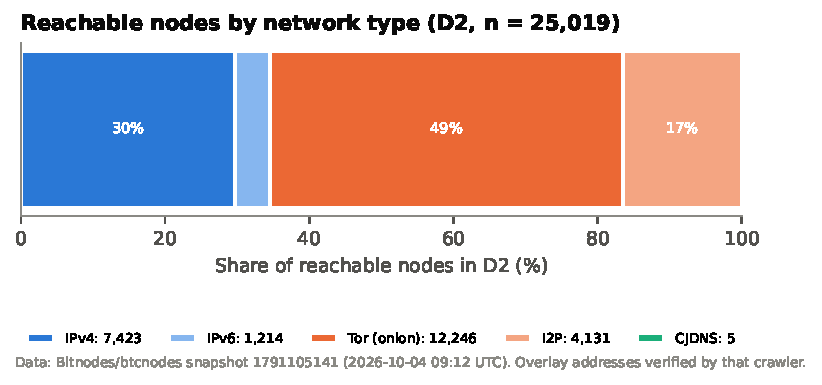
\includegraphics[width=0.85\linewidth]{networks.pdf}
\caption{Reachable nodes by network type (D2). Only the IPv4 and IPv6 parts can be attributed to ASes, providers or countries.}\label{fig:networks}
\end{figure}

One group of nodes stands out. \FleetN{} IPv4 endpoints in D2, or \FleetShareIP{} of its IP hosts, look exactly alike: user agent \texttt{/Satoshi:27.0.0/}, service bits 3077 (without \texttt{NODE\_\allowbreak{}WITNESS}) and a reported height of 0. All \FleetLinode{} are on Akamai/Linode, spread over \FleetSubnets{} /24 subnets and \FleetNetgroups{} /16 netgroups. KIT's dossier contains only \FleetKIT{} endpoints with this fingerprint. Our home crawl came across \FleetDoneSeen{} of the addresses in gossip, and the AWS crawl \FleetAwsSeen{}, all of which completed a handshake. A genuine Bitcoin Core 27.0 node always announces \texttt{NODE\_\allowbreak{}WITNESS}, so we think the fleet is most likely run by a single party for some purpose other than serving the network. It matters for the results: counted as ordinary nodes, it makes Akamai/Linode the largest provider in D2 (\DtwoProvTopone), whereas without it \DtwoFProvToponeLabel{} is the largest (\DtwoFProvTopone). A study based on one crawler alone would have no way of noticing this.

\subsection{Reachable nodes follow more than one chain}\label{sec:chain}

Table~\ref{tab:chainview} groups all reachable D2 hosts by the start height they report during the handshake. \Chaintip{} hosts (\ChaintipShare) are within six blocks of the most common height, \ObservedTip. Another \Chainabovetip{} (\ChainabovetipShare) report heights far above it, by a median of \AboveMedian{} blocks; \ChainAboveKnots{} of them run Bitcoin Knots, nearly all version 29.4.1 or 29.4.2. A further \ChainstalledNineSixOnek{} (\ChainstalledNineSixOnekShare) report heights between 961{,}600 and 961{,}700 (median \StalledMedian), and almost all of these run Knots 29.3 or 29.4.0 or a BIP-110 build. Our own crawls show the same pattern: \DoneAbove{} nodes above the tip and \DoneStalled{} near 961{,}6xx from home, and \DonebAbove{} and \DonebStalled{} among the IPv4 nodes seen from AWS.

\begin{table}[t]
\centering\small
\caption{Start height reported in the version handshake by all reachable nodes in D2 (IPv4, IPv6, Tor, I2P, CJDNS; unique hosts), relative to the modal height of the snapshot.}
\label{tab:chainview}

\begin{tabular}{lrrrrr}
\toprule
Height relative to SHA256d tip & Bitcoin Core & Bitcoin Knots & other & Total & Share (\%) \\
\midrule
at tip ($\pm$6 blocks) & 19820 & 2284 & 64 & 22168 & 88.6 \\
below tip (lagging/syncing) & 188 & 17 & 5 & 210 & 0.8 \\
above tip ($>$6 blocks) & 1 & 1068 & 1 & 1070 & 4.3 \\
961{,}600--961{,}700 & 4 & 716 & 0 & 720 & 2.9 \\
zero & 849 & 0 & 2 & 851 & 3.4 \\
\bottomrule
\end{tabular}
\end{table}


According to the Knots release notes, version 29.4.1 introduces a backward-incompatible switch to a BLAKE2b proof of work, and version 29.3 adds the BIP-110 ``Reduced Data Temporary Softfork'' \cite{knots2026notes}. Press reports describe a BIP-110 chain that stopped after splitting off in August 2026 \cite{cryptoslate2026knots}. Heights far ahead of the SHA256d tip and heights frozen near 961{,}6xx fit nodes following these two chains. We did not validate the chains ourselves, so this reading rests on the release notes and on the heights the nodes report.

Either way, several thousand reachable nodes enforce rules that the dominant chain does not, and every crawler counts them anyway. They also use the same infrastructure: \ForkProvBoth{} of the \ForkProvTotal{} providers that host the \ForkIP{} forked IPv4/IPv6 nodes also host main-chain nodes, and \ForkInTopTen{} of the forked nodes sit at one of the ten largest main-chain providers, although they are more often on access networks (\ForkResid{} against \MainResid). Where a node is hosted tells us nothing about which chain it validates, which is also why a node count is not a measure of consensus.

\subsection{Geographic distribution}

Functional D2 nodes are located in \DtwoFCcGroups{} countries. The \CcOneName{} has \CcOneShare{} of them, followed by \CcTwoName{} with \CcTwoShare{} and \CcThreeName{} with \CcThreeShare{}. The five largest countries hold \DtwoFCcTopfive{} of nodes, the country HHI is \DtwoFCcHHI{} and $N_{50}=\DtwoFCcNfifty$ (Fig.~\ref{fig:country}). By registration rather than geolocation, the \DtwoFCcToponeLabel{} share rises to \DtwoFRirTopone{} (HHI \DtwoFRirHHI), and KIT, which records the country in which an AS is registered, gives \DthreeFCcTopone{} (HHI \DthreeFCcHHI).

Country is the most concentrated dimension we measured: the two largest countries together hold \CcTopTwo{} of attributable nodes, and \DtwoFCcNfifty{} countries are enough to reach half. The country of a node is itself uncertain, though. Geolocation and registration agree for \GeoAgree{} of nodes overall but for only \GeoAgreeHone{} of nodes in cloud ranges, compared with \GeoAgreeR{} for residential nodes, because cloud address space registered in one country is often used in another.

\begin{figure}[t]\centering
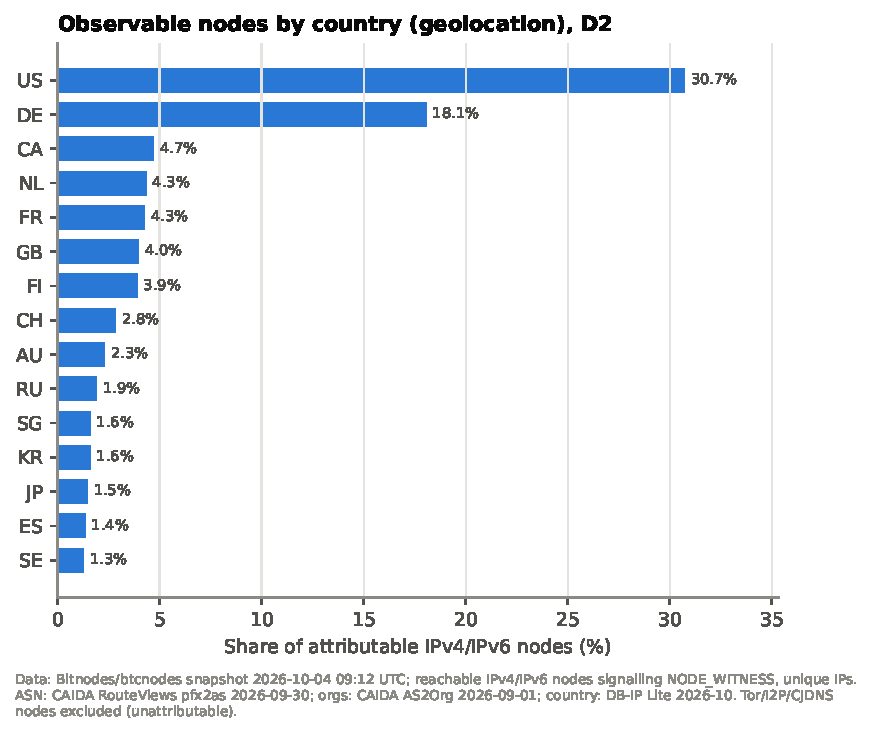
\includegraphics[width=0.75\linewidth]{dist_country.pdf}
\caption{Functional IPv4/IPv6 nodes by geolocated country (D2).}\label{fig:country}
\end{figure}

\subsection{ASes and providers}

Functional D2 nodes are spread over \DtwoFAsnGroups{} ASNs and \DtwoFProvGroups{} providers (Table~\ref{tab:concentration}, Figs.~\ref{fig:provider}--\ref{fig:cumulative}). \ProvOneName{} hosts \ProvOneShare{} of them, followed by \ProvTwoName{} (\ProvTwoShare), \ProvThreeName{} (\ProvThreeShare), \ProvFourName{} (\ProvFourShare) and \ProvFiveName{} (\ProvFiveShare); Table~\ref{tab:topprov} lists the ten largest, which together host \DtwoFProvTopten{}. The provider HHI is \DtwoFProvHHI{} ($N_\text{eff}=\DtwoFProvNeff$), the ASN HHI is \DtwoFAsnHHI{} ($N_\text{eff}=\DtwoFAsnNeff$, see also Fig.~\ref{fig:asn}), and half of the attributable nodes are covered by $N_{50}=\DtwoFProvNfifty$ providers or \DtwoFAsnNfifty{} ASNs. KIT's data give almost the same picture, with \DthreeFProvToponeLabel{} at \DthreeFProvTopone, a provider HHI of \DthreeFProvHHI, an ASN HHI of \DthreeFAsnHHI{} and $N_{50}=\DthreeFProvNfifty$ (Fig.~\ref{fig:hhigini}). The Gini coefficient across providers is high (\DtwoFProvGini) because of the long tail of providers that host only one node.

These numbers support H1, with a qualification. Concentration is clearly there, since \DtwoFProvNfifty{} providers host half of the attributable nodes and the largest one hosts about one in ten. In absolute terms, however, it is moderate. The provider and AS HHIs are far below the 1{,}800 reference level, while the country HHI comes close to it under geolocation and exceeds it under KIT's registration-based country. The high Gini and the moderate HHI describe the same situation from two sides: many very small groups next to a handful of medium-sized ones, and no group that dominates.

\begin{table}[t]
\centering\small
\caption{Concentration of observable IPv4/IPv6 nodes (suffix f: NODE\_WITNESS nodes only). Top-k shares in \% of attributable nodes; N\_eff = 10{,}000/HHI; N50 = smallest number of groups jointly holding at least 50\% of attributable nodes.}
\label{tab:concentration}
\resizebox{\linewidth}{!}{%
\begin{tabular}{llrrrrrrrrr}
\toprule
Data & Dimension & n & Groups & Top-1 & Top-5 & Top-10 & HHI & N\_eff & Gini & N50 \\
\midrule
D1 & Country (geolocation, DB-IP) & 4804 & 82 & 27.5 & 60.8 & 76.7 & 1268 & 7.9 & 0.8 & 3 \\
D1 & ASN & 4804 & 864 & 12.4 & 35.0 & 44.8 & 336 & 29.8 & 0.8 & 15 \\
D1 & Organisation (CAIDA AS2Org) & 4804 & 803 & 12.7 & 35.9 & 46.6 & 356 & 28.1 & 0.8 & 13 \\
D1 & Provider (sibling-merged) & 4804 & 780 & 12.7 & 36.5 & 48.7 & 373 & 26.8 & 0.8 & 11 \\
D1b & Country (geolocation, DB-IP) & 8685 & 92 & 30.6 & 61.7 & 76.4 & 1373 & 7.3 & 0.8 & 3 \\
D1b & ASN & 8685 & 1285 & 10.2 & 29.4 & 40.8 & 247 & 40.6 & 0.8 & 21 \\
D1b & Organisation (CAIDA AS2Org) & 8685 & 1195 & 10.4 & 30.5 & 42.7 & 267 & 37.5 & 0.8 & 16 \\
D1b & Provider (sibling-merged) & 8685 & 1166 & 10.4 & 31.3 & 45.2 & 288 & 34.7 & 0.8 & 13 \\
D2 & Country (geolocation, DB-IP) & 8637 & 94 & 31.6 & 64.8 & 78.8 & 1491 & 6.7 & 0.8 & 2 \\
D2 & ASN & 8637 & 1264 & 10.2 & 31.4 & 42.9 & 287 & 34.8 & 0.8 & 18 \\
D2 & Organisation (CAIDA AS2Org) & 8637 & 1169 & 10.2 & 32.3 & 44.8 & 304 & 32.9 & 0.8 & 14 \\
D2 & Provider (sibling-merged) & 8637 & 1138 & 10.2 & 32.9 & 47.0 & 320 & 31.2 & 0.8 & 12 \\
D3 & Country (AS registration, KIT whois) & 8946 & 96 & 39.2 & 71.2 & 80.6 & 2002 & 5.0 & 0.9 & 2 \\
D3 & ASN & 8924 & 1300 & 9.8 & 27.3 & 38.6 & 219 & 45.6 & 0.8 & 25 \\
D3 & Organisation (CAIDA AS2Org) & 8924 & 1197 & 10.1 & 28.3 & 40.8 & 239 & 41.8 & 0.8 & 19 \\
D3 & Provider (sibling-merged) & 8924 & 1168 & 10.1 & 29.3 & 43.6 & 262 & 38.2 & 0.8 & 14 \\
D1f & Country (geolocation, DB-IP) & 4743 & 82 & 27.4 & 60.5 & 76.4 & 1259 & 7.9 & 0.8 & 3 \\
D1f & ASN & 4743 & 863 & 12.6 & 35.4 & 45.2 & 341 & 29.3 & 0.7 & 16 \\
D1f & Organisation (CAIDA AS2Org) & 4743 & 802 & 12.8 & 36.3 & 47.2 & 361 & 27.7 & 0.8 & 12 \\
D1f & Provider (sibling-merged) & 4743 & 779 & 12.8 & 36.9 & 49.2 & 379 & 26.4 & 0.8 & 11 \\
D1bf & Country (geolocation, DB-IP) & 8523 & 92 & 30.4 & 61.2 & 76.1 & 1355 & 7.4 & 0.8 & 3 \\
D1bf & ASN & 8523 & 1283 & 10.3 & 29.9 & 40.7 & 250 & 39.9 & 0.8 & 22 \\
D1bf & Organisation (CAIDA AS2Org) & 8523 & 1193 & 10.6 & 31.0 & 43.3 & 272 & 36.8 & 0.8 & 17 \\
D1bf & Provider (sibling-merged) & 8523 & 1164 & 10.6 & 31.8 & 45.9 & 293 & 34.1 & 0.8 & 13 \\
D2f & Country (geolocation, DB-IP) & 7771 & 94 & 30.7 & 62.1 & 77.0 & 1397 & 7.2 & 0.8 & 3 \\
D2f & ASN & 7771 & 1261 & 10.7 & 26.8 & 38.1 & 226 & 44.3 & 0.8 & 26 \\
D2f & Organisation (CAIDA AS2Org) & 7771 & 1166 & 11.0 & 27.8 & 40.5 & 247 & 40.6 & 0.8 & 20 \\
D2f & Provider (sibling-merged) & 7771 & 1135 & 11.0 & 28.8 & 43.3 & 267 & 37.5 & 0.8 & 15 \\
D3f & Country (AS registration, KIT whois) & 8861 & 95 & 39.1 & 71.2 & 80.6 & 1997 & 5.0 & 0.9 & 2 \\
D3f & ASN & 8839 & 1294 & 9.8 & 27.5 & 38.7 & 221 & 45.3 & 0.8 & 25 \\
D3f & Organisation (CAIDA AS2Org) & 8839 & 1191 & 10.1 & 28.4 & 41.0 & 241 & 41.5 & 0.8 & 19 \\
D3f & Provider (sibling-merged) & 8839 & 1162 & 10.1 & 29.5 & 43.7 & 264 & 37.9 & 0.8 & 14 \\
\bottomrule
\end{tabular}}
\end{table}


\begin{figure}[t]\centering
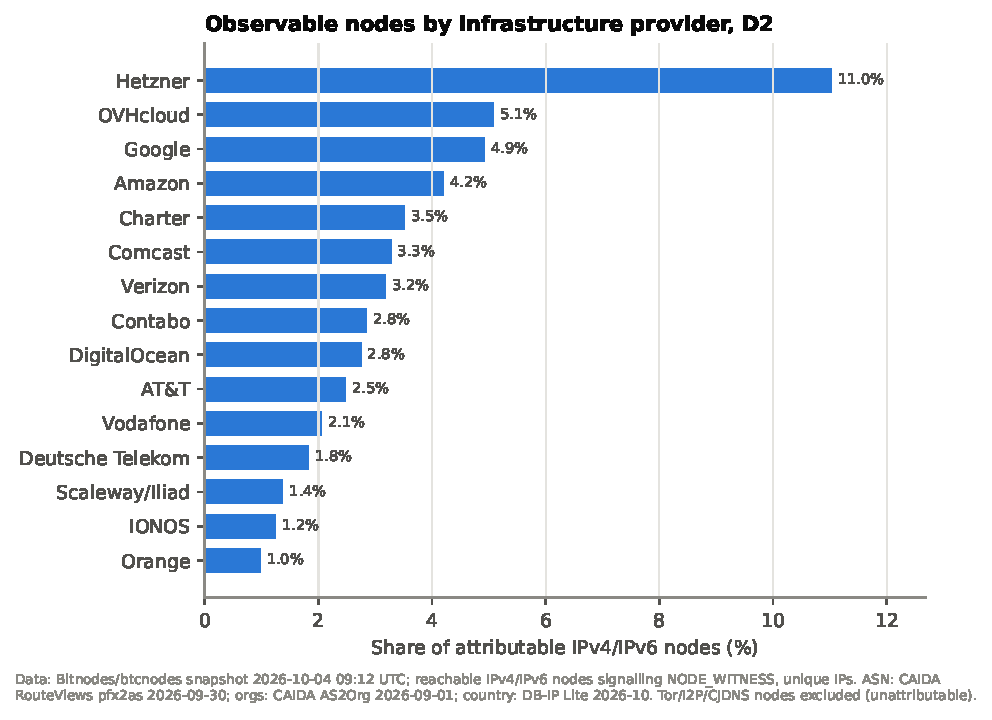
\includegraphics[width=0.75\linewidth]{dist_provider.pdf}
\caption{Functional IPv4/IPv6 nodes by provider (sibling-merged CAIDA organisations), D2.}\label{fig:provider}
\end{figure}

\begin{figure}[t]\centering
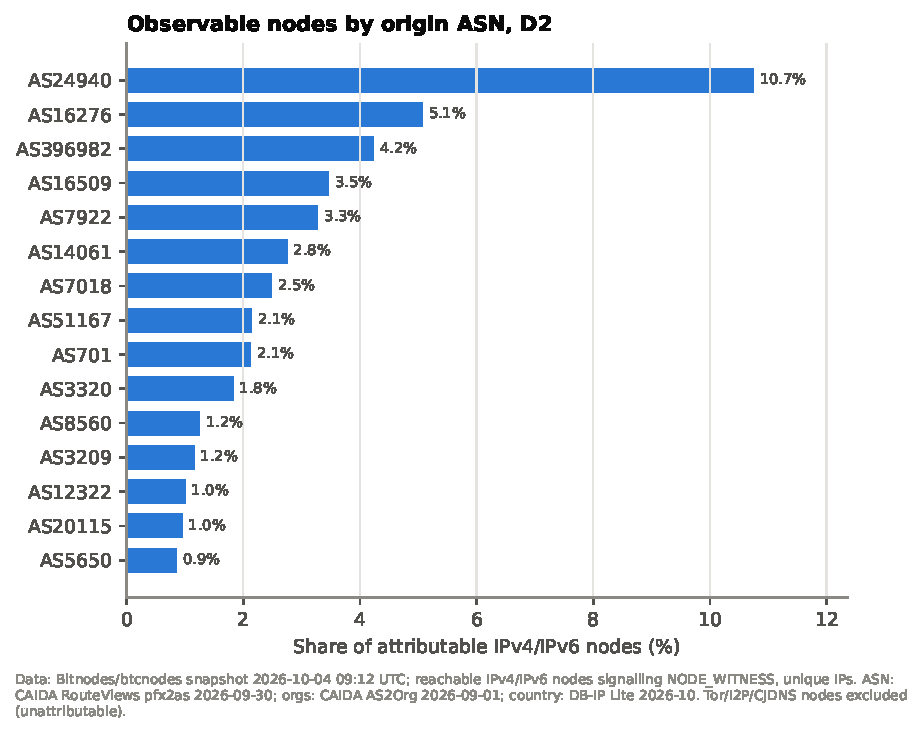
\includegraphics[width=0.75\linewidth]{dist_asn.pdf}
\caption{Functional IPv4/IPv6 nodes by origin ASN, D2.}\label{fig:asn}
\end{figure}

\begin{figure}[t]\centering
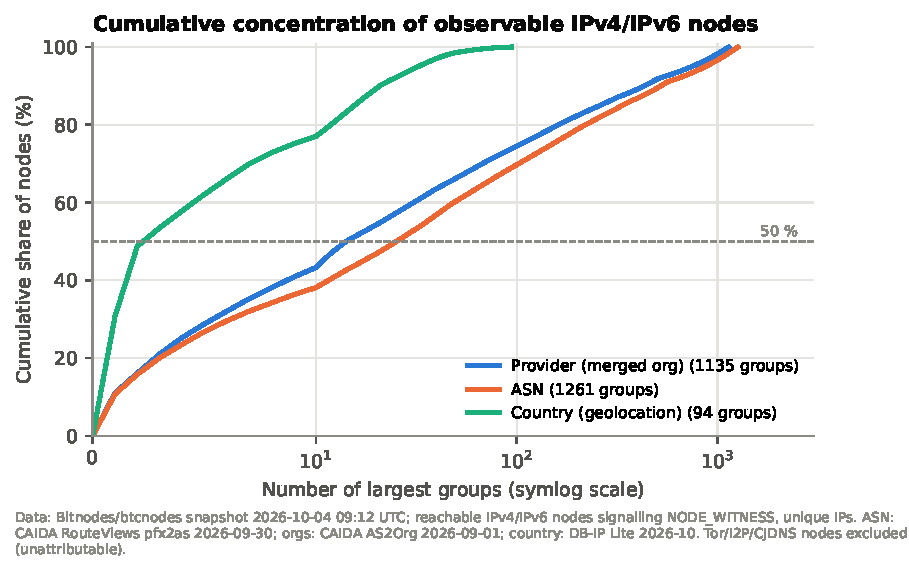
\includegraphics[width=0.75\linewidth]{cumulative_concentration.pdf}
\caption{Cumulative share of functional IPv4/IPv6 nodes held by the $k$ largest providers, ASNs and countries (D2).}\label{fig:cumulative}
\end{figure}

\begin{figure}[t]\centering
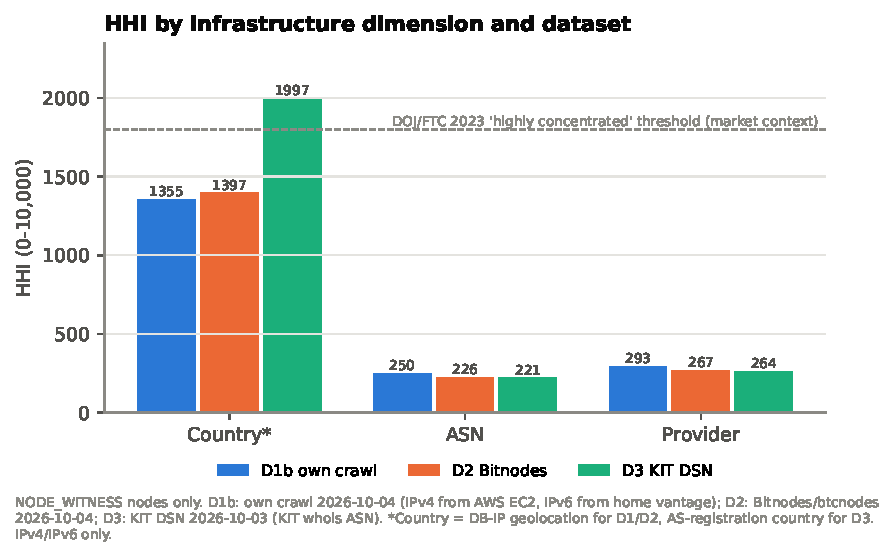
\includegraphics[width=0.49\linewidth]{hhi_comparison.pdf}\hfill
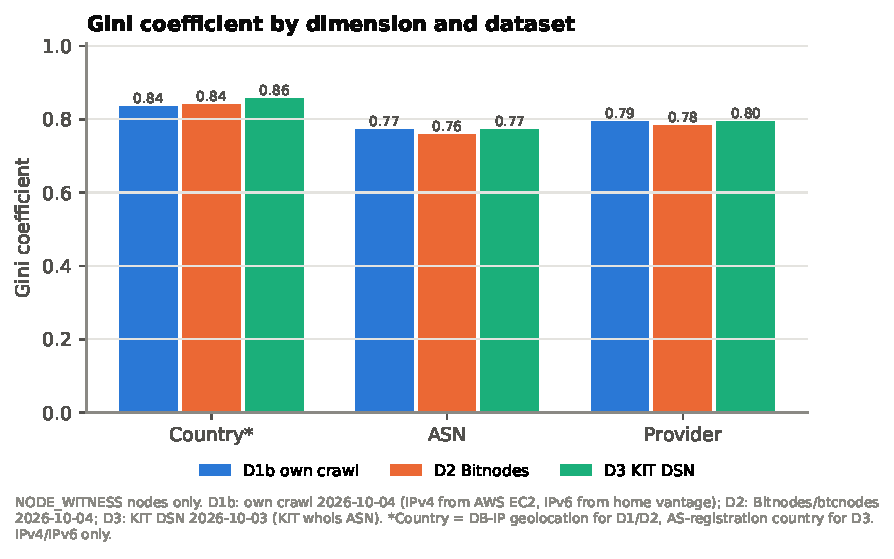
\includegraphics[width=0.49\linewidth]{gini_comparison.pdf}
\caption{HHI and Gini coefficient per dimension for the three datasets (functional nodes). The dashed line marks the 1{,}800 HHI reference of \cite{doj2023merger}.}\label{fig:hhigini}
\end{figure}

\begin{table}[t]
\centering\small
\caption{Ten largest infrastructure providers (sibling-merged CAIDA organisations) among functional (NODE\_WITNESS) IPv4/IPv6 nodes in D2.}
\label{tab:topprov}

\begin{tabular}{lrrr}
\toprule
Group & Nodes & Share (\%) & Cum. (\%) \\
\midrule
Hetzner & 857 & 11.0 & 11.0 \\
OVHcloud & 395 & 5.1 & 16.1 \\
Google & 383 & 4.9 & 21.0 \\
Amazon & 327 & 4.2 & 25.2 \\
Charter & 273 & 3.5 & 28.8 \\
Comcast & 255 & 3.3 & 32.0 \\
Verizon & 247 & 3.2 & 35.2 \\
Contabo & 221 & 2.8 & 38.1 \\
DigitalOcean & 214 & 2.8 & 40.8 \\
AT\&T & 193 & 2.5 & 43.3 \\
\bottomrule
\end{tabular}
\end{table}


\subsection{Hosting and residential connections}

Of the functional D2 nodes, \DtwoFClassHOne{} lie in published cloud ranges (H1), \DtwoFClassHTwo{} in hosting ASes (H2) and \DtwoFClassR{} in access networks (R), while \DtwoFClassU{} could not be classified (Table~\ref{tab:classes}, Fig.~\ref{fig:classes}). The hosted share is therefore somewhere between \DtwoFHostedLow{} and \DtwoFHostedHigh. KIT's data, which can only be classified at the AS level, give \DthreeFHostedCentral{} hosted and \DthreeFClassR{} residential.

So a large minority of attributable nodes, probably a little under half, runs on commercial hosting, and roughly half runs on home or small-business connections. The R class is an inference made at the AS level; a node in an access network can still sit in a company's server room, and a node at a small VPS provider that is missing from our lists ends up in U. Our name-based rule matched \RegexNodes{} nodes (\RegexShare), including some false positives such as ISP names that contain ``colo'', so its effect on the central estimate is at most that large.

\begin{table}[t]
\centering\small
\caption{Infrastructure class of attributable IPv4/IPv6 nodes (\% of nodes). D3 has no IP addresses, so H1 (published cloud ranges) cannot be applied there; its cloud nodes fall into H2.}
\label{tab:classes}
\resizebox{\linewidth}{!}{%
\begin{tabular}{lrrrrrrrr}
\toprule
Data & n & H1 & H2 & R & U & Hosted low & Hosted central & Hosted high \\
\midrule
D1 & 4804 & 19.5 & 32.7 & 42.0 & 5.7 & 19.5 & 52.2 & 58.0 \\
D1b & 8685 & 17.8 & 29.2 & 47.3 & 5.6 & 17.8 & 47.0 & 52.7 \\
D2 & 8637 & 20.9 & 27.8 & 45.8 & 5.5 & 20.9 & 48.7 & 54.2 \\
D3 & 8959 & 0.0 & 42.1 & 51.7 & 5.7 & 0.0 & 42.1 & 47.9 \\
D1f & 4743 & 18.6 & 33.0 & 42.6 & 5.8 & 18.6 & 51.7 & 57.4 \\
D1bf & 8523 & 16.5 & 29.6 & 48.2 & 5.7 & 16.5 & 46.1 & 51.8 \\
D2f & 7771 & 12.3 & 30.8 & 50.9 & 6.0 & 12.3 & 43.1 & 49.1 \\
D3f & 8874 & 0.0 & 42.1 & 51.8 & 5.7 & 0.0 & 42.1 & 47.8 \\
\bottomrule
\end{tabular}}
\end{table}


\begin{figure}[t]\centering
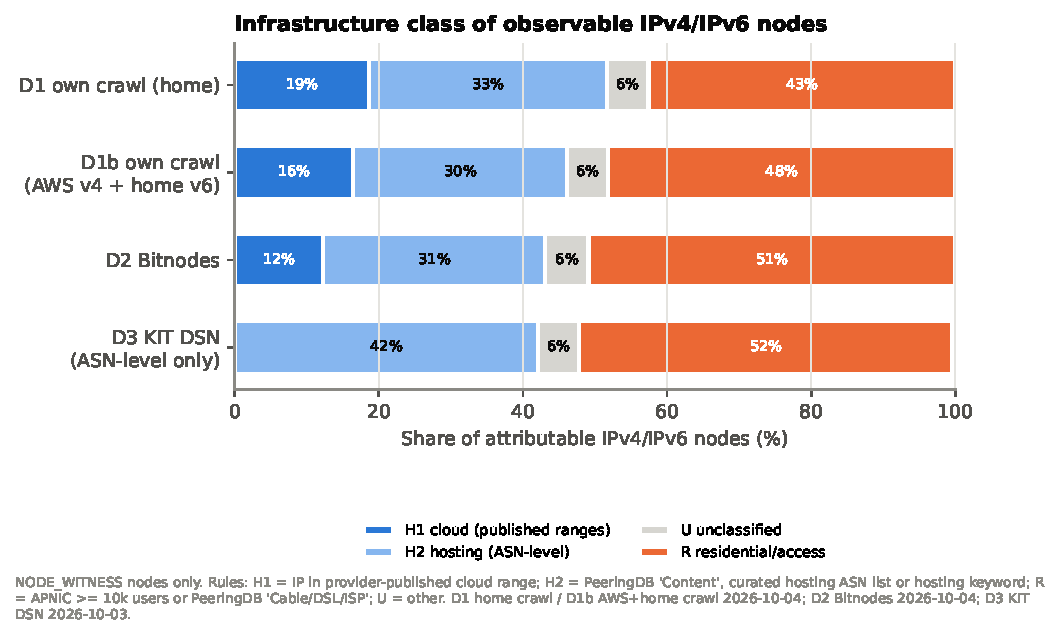
\includegraphics[width=0.8\linewidth]{infra_classes.pdf}
\caption{Infrastructure class of functional IPv4/IPv6 nodes.}\label{fig:classes}
\end{figure}

\subsection{Client software}

Bitcoin Core runs on \DtwoFCoreShare{} of functional IP nodes. Bitcoin Knots accounts for \KnotsShareAll{} of all reachable hosts and \KnotsShareOverlay{} of the Tor and I2P hosts, and it is far more common on residential addresses (\KnotsShareR) than in cloud ranges (\KnotsShareHone). By the HHI, client diversity is low (\DtwoFClientHHI). The minority client has grown quickly, though: in KIT's data it stayed below one percent until 2024 and reached \TSTwentySixKnots{} in 2026. Since that client is now also the one behind the chain splits described in \S\ref{sec:chain}, more software diversity has in this case come with less agreement on the rules.

\subsection{Change over time}

In KIT's annual snapshots (Table~\ref{tab:timeseries}, Fig.~\ref{fig:time}), the ASN HHI went from \TSFifteenAsnHHI{} in 2015 up to \TSPeakHHI{} in \TSPeakYear{} and back down to \TSTwentySixAsnHHI{} in 2026. The share of peers in hosting ASes peaked at \TSPeakHosted{} in \TSPeakHostedYear{} and is now \TSTwentySixHosted{}. \TSTwentySixProvTopLabel{} has been the largest provider in every year since 2016. Over the seven days before our crawl, none of the KIT metrics moved by more than \StabMaxRel{} relative to its mean, so our snapshot is not an unusual day. Over the longer run, concentration of the reachable network has not simply kept rising; by these measures it is lower today than in 2020--2022.

\begin{table}[t]
\centering\small
\caption{Infrastructure diversity of peers in KIT DSN dossiers (1 October of each year, IPv4/IPv6). Hosted \% = share of peers in ASNs classified as hosting (H2) with 2026 classification sources.}
\label{tab:timeseries}
\resizebox{\linewidth}{!}{%
\begin{tabular}{lrrrrlrrlrr}
\toprule
Date & Peers & ASNs & ASN HHI & Top-10 ASN \% & Top provider & \% & Hosted \% & Top AS-cc & \% & Knots \% \\
\midrule
2015-10-01 & 4934 & 1032 & 149 & 29.7 & Comcast & 7.7 & 29.4 & US & 39.1 & 0.0 \\
2016-10-01 & 5419 & 941 & 203 & 34.8 & Hetzner & 8.3 & 43.5 & US & 33.8 & 0.5 \\
2017-10-02 & 8868 & 1224 & 249 & 39.4 & Hetzner & 10.5 & 51.6 & US & 33.9 & 0.5 \\
2018-10-01 & 10158 & 1312 & 263 & 42.1 & Hetzner & 9.8 & 52.7 & US & 33.0 & 0.4 \\
2019-10-01 & 10021 & 1192 & 333 & 46.0 & Hetzner & 12.0 & 57.6 & US & 38.6 & 0.2 \\
2020-10-01 & 8843 & 1083 & 408 & 50.5 & Hetzner & 13.4 & 61.3 & US & 36.5 & 0.4 \\
2021-10-01 & 9858 & 1223 & 358 & 46.2 & Hetzner & 13.3 & 53.9 & US & 39.1 & 0.3 \\
2022-10-01 & 7679 & 1001 & 390 & 47.7 & Hetzner & 12.5 & 53.5 & US & 40.2 & 0.5 \\
2023-10-01 & 6895 & 985 & 293 & 42.1 & Hetzner & 12.8 & 50.2 & US & 36.7 & 0.3 \\
2024-10-01 & 7804 & 1104 & 265 & 41.0 & Hetzner & 12.3 & 50.1 & US & 37.3 & 0.8 \\
2025-10-01 & 9886 & 1324 & 228 & 40.7 & Hetzner & 9.7 & 43.9 & US & 39.3 & 9.9 \\
2026-10-01 & 9011 & 1309 & 219 & 38.5 & Hetzner & 10.0 & 42.4 & US & 39.1 & 11.4 \\
\bottomrule
\end{tabular}}
\end{table}


\begin{figure}[t]\centering
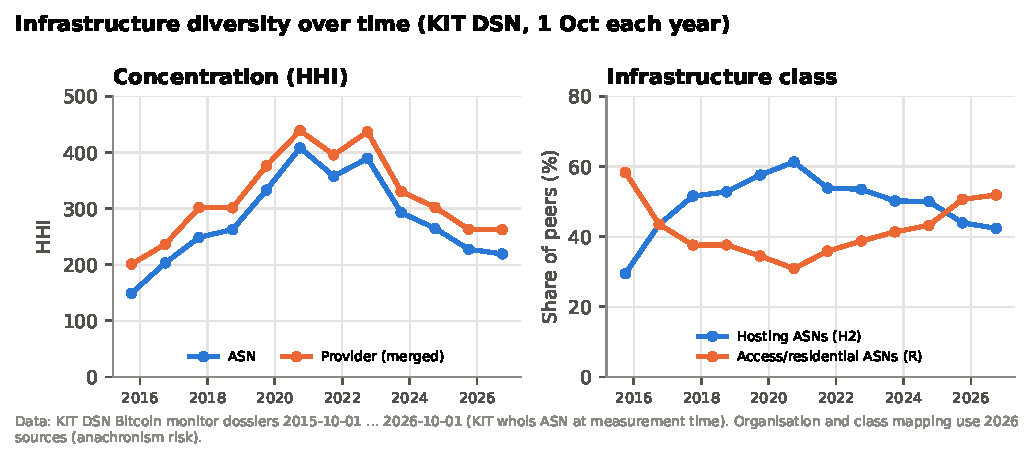
\includegraphics[width=0.9\linewidth]{diversity_over_time.pdf}
\caption{Infrastructure diversity over time (KIT DSN). Organisation and class mapping use 2026 sources.}\label{fig:time}
\end{figure}

\subsection{Agreement between datasets}

The AWS crawl reached \AwsCoverDtwoVfour{} of the IPv4 hosts listed by D2, against \HomeCoverDtwoVfour{} for the home crawl, and it found \AwsOnlyVfour{} IPv4 hosts that D2 does not list. D1b and D2 share \OverlapbBoth{} IPs, with \OverlapbOnlyDone{} seen only by D1b and \OverlapbOnlyDtwo{} only by D2, a Jaccard similarity of \OverlapbJaccard{} (\OverlapJaccard{} for the home crawl alone). For functional nodes, D1b identifies the same largest provider (\DonebFProvToponeLabel{} at \DonebFProvTopone) and gives a provider HHI of \DonebFProvHHI{}, an ASN HHI of \DonebFAsnHHI{}, $N_{50}=\DonebFProvNfifty$ providers, a country HHI of \DonebFCcHHI{} and a central hosted share of \DonebFHostedCentral{}, with \DonebFClassR{} residential. The home crawl alone, affected by NAT, gives a higher provider HHI (\DoneFProvHHI) and a higher hosted share (\DoneFHostedCentral), as expected from its bias (\S\ref{sec:threats}). Three crawlers with different code, vantage points and discovery methods thus agree closely on who the largest provider is, on its share and on the provider and ASN HHIs, so the concentration figures do not depend on one particular crawler.

\subsection{A second measurement day}\label{sec:twodays}

On 6 October we repeated the Bitnodes snapshot and the AWS crawl; the AWS machine again had no IPv6, so that comparison covers IPv4 only (Table~\ref{tab:twodays}). The concentration figures hardly changed. In Bitnodes, \TdDtwoBTopLabel{} went from \TdDtwoATop{} to \TdDtwoBTop{} and the provider HHI from \TdDtwoAProvHHI{} to \TdDtwoBProvHHI{}, and the hosted share moved from \TdDtwoAHosted{} to \TdDtwoBHosted{}. In the AWS crawl the provider HHI was \TdAwsAProvHHI{} on both days. Across both datasets the provider HHI changed by at most \TdMaxProvHHIChange{} points.

The node population itself turned over more. Of the functional IP nodes in the first AWS crawl, \TdAwsRetained{} were reachable again two days later, while \TdAwsOnlyB{} nodes appeared that had not been seen before. Hosted nodes were more stable (\TdAwsRetHosted{} seen again) than nodes on access networks (\TdAwsRetR). Bitnodes shows a lower overall retention of \TdDtwoRetained{} and a less clear pattern by class (\TdDtwoRetHOne{} for H1, \TdDtwoRetHTwo{} for H2, \TdDtwoRetR{} for R), which may partly reflect day-to-day differences in what its crawler reaches. Either way, individual nodes come and go noticeably faster than the overall distribution changes.

The Linode fleet shrank from \TdDtwoAFleet{} to \TdDtwoBFleet{} endpoints in Bitnodes, \TdFleetBoth{} of which had the same addresses on both days. The number of nodes reporting heights above the SHA256d tip rose slightly, from \TdDtwoAAbove{} to \TdDtwoBAbove{} (AWS crawl: \TdAwsAAbove{} to \TdAwsBAbove), while the number stuck near 961{,}6xx stayed flat (\TdDtwoAStalled{} and \TdDtwoBStalled).

\begin{table}[t]
\centering\small
\caption{The same measurements on 4 and 6 October 2026 (functional IPv4/IPv6 nodes for D2, functional IPv4 nodes for the AWS crawl). Hosted \% is the central estimate H1+H2.}
\label{tab:twodays}
\resizebox{\linewidth}{!}{%
\begin{tabular}{llrlrrrrrr}
\toprule
Dataset & Day & IP nodes & Top provider & Top \% & Top-5 \% & Prov. HHI & ASN HHI & Country HHI & Hosted \% \\
\midrule
Bitnodes (D2) & 4 Oct & 7771 & Hetzner & 11.0 & 28.8 & 267 & 226 & 1397 & 43.1 \\
Bitnodes (D2) & 6 Oct & 7792 & Hetzner & 10.8 & 28.4 & 261 & 220 & 1387 & 42.6 \\
AWS crawl, IPv4 (D1b) & 4 Oct & 6796 & Hetzner & 8.3 & 26.2 & 221 & 177 & 1474 & 40.1 \\
AWS crawl, IPv4 (D1b) & 6 Oct & 6842 & Hetzner & 8.3 & 26.2 & 221 & 176 & 1478 & 39.8 \\
\bottomrule
\end{tabular}}
\end{table}


% =====================================================================
\section{Failure scenarios}\label{sec:failure}

\paragraph{Counting the losses.} Table~\ref{tab:failstatic} and Fig.~\ref{fig:failstatic} start from the \FailIP{} functional IPv4/IPv6 nodes in D2 that are on the SHA256d chain. If \ProvOneName{} went offline, \FailProvLost{} of them would disappear. That is \FailProvIP{} of the IP-reachable nodes and \FailProvAll{} of all reachable nodes; relative to the whole network including the D4 estimate, it is between \FailProvA{} (if non-listening nodes are unaffected) and \FailProvB{} (if they are affected in the same proportion). Losing the top-5 providers would remove \FailTopfiveIP{} of IP-reachable nodes, losing the \CcOneName{} \FailCcIP{}, and losing every hosted node \FailHostedIP{}. Even then, at least \FailMinAsns{} ASNs and \FailMinCcs{} countries would still have nodes.

\begin{table}[t]
\centering\small
\caption{Static accounting of hypothetical failures (D2, SHA256d-chain functional IPv4/IPv6 nodes). \% all (A): non-listening nodes (Luke Dashjr estimate) assumed unaffected; (B): affected in the same proportion as reachable IP nodes.}
\label{tab:failstatic}
\resizebox{\linewidth}{!}{%
\begin{tabular}{lrrrrrrr}
\toprule
Scenario & Lost & \% IP & \% reach. & \% all (A) & \% all (B) & ASNs left & Countries left \\
\midrule
Baseline (no failure) & 0 & 0.0 & 0.0 & 0.0 & 0.0 & 1209 & 94 \\
Largest ASN (AS24940) & 821 & 11.3 & 3.7 & 0.6 & 9.9 & 1208 & 94 \\
Largest provider (Hetzner) & 842 & 11.5 & 3.8 & 0.7 & 10.2 & 1205 & 94 \\
Largest country (US) & 2159 & 29.6 & 9.7 & 1.7 & 26.1 & 954 & 93 \\
Top-5 providers & 2154 & 29.5 & 9.6 & 1.7 & 26.1 & 1186 & 94 \\
Top-10 providers & 3194 & 43.8 & 14.3 & 2.5 & 38.6 & 1175 & 94 \\
All hosted (H1+H2) & 3220 & 44.2 & 14.4 & 2.5 & 38.9 & 1002 & 92 \\
\bottomrule
\end{tabular}}
\end{table}


\begin{figure}[t]\centering
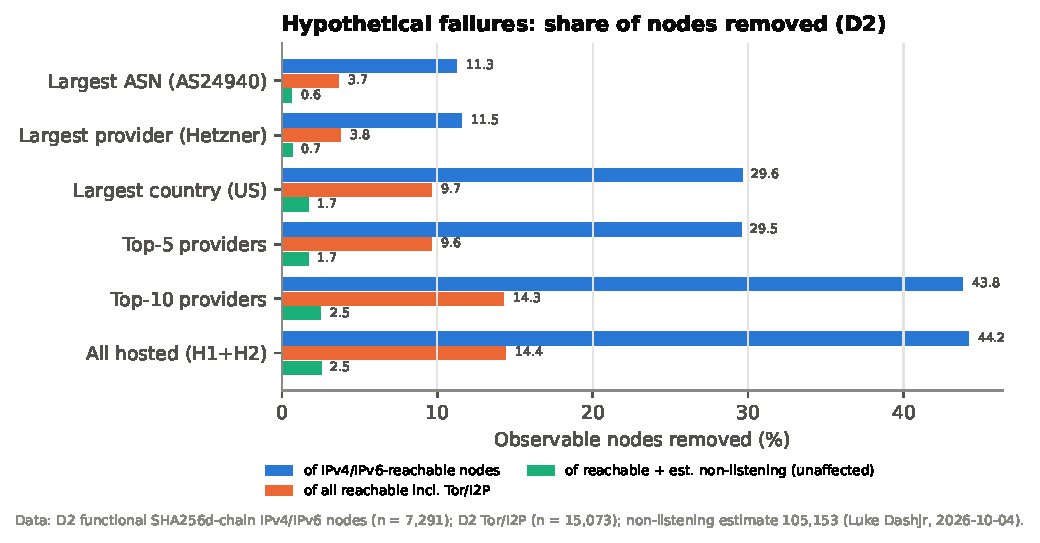
\includegraphics[width=0.8\linewidth]{failure_scenarios.pdf}
\caption{Share of nodes removed in each hypothetical scenario, under three denominators.}\label{fig:failstatic}
\end{figure}

\paragraph{Connectivity in the model.} With the D4 estimate included, a message needs \ModUBaseHops{} hops on average to reach a node in the model network (\ModUBaseFullHops{} over full-relay links only). Each reachable node receives \ModUBaseInbound{} inbound connections on average and at most \ModUBaseMaxInbound, against a default capacity of about \InboundCap{}. Removing every hosted node at once leaves \ModUHostedZero{} of the remaining nodes without any outbound peer and \ModUHostedZeroFull{} without a full-relay peer, and the largest connected component still contains \ModUHostedLCC{} of them. The average path grows to \ModUHostedHops{} hops before nodes reconnect and falls to \ModUHostedHopsAfter{} afterwards. In no scenario do more than \ModUMaxZero{} of nodes lose all outbound peers, and the LCC never drops below \ModUMinLCC. If we assume that no node uses both clearnet and an overlay network, the LCC after losing all hosted nodes is \ModZeroDualHostedLCC{}, but it is already \ModZeroDualBaseLCC{} without any failure, because under that assumption the Tor- and I2P-only nodes form a separate network from the start (Fig.~\ref{fig:failmodel}).

\paragraph{Inbound capacity.} Since only reachable nodes accept connections, they have to absorb the outbound connections of all other nodes. Table~\ref{tab:capacity} shows what share of the outbound demand would exceed the inbound slots of the nodes it is aimed at. Without non-listening nodes this never happens (\UnmetReachOnlyMax). With the D4 estimate and the \InboundCap{} slots of released versions, \UnmetRelBase{} of the demand cannot be served even when nothing has failed. Losing the largest provider raises this to \UnmetRelProv, losing the top-5 providers or the largest country to about \UnmetRelTopfive, and losing all hosted nodes to \UnmetRelHosted. With master's \InboundCapMaster{} slots the corresponding figures are \UnmetMasBase, \UnmetMasProv, \UnmetMasTopfive{} and \UnmetMasHosted. A node that is turned away would try other peers, so these numbers describe how much pressure the remaining nodes are under rather than how many connections are lost for good.

\begin{table}[t]\centering\small
\caption{Share of outbound connection demand exceeding inbound capacity (model, including the D4 non-listening estimate, mean of three seeds).}\label{tab:capacity}
\begin{tabular}{lrr}
\toprule
Scenario & Released v27--v31 (\InboundCap{} slots) & Master (\InboundCapMaster{} slots)\\
\midrule
Baseline (no failure) & \UnmetRelBase & \UnmetMasBase\\
Largest ASN & \UnmetRelAsn & \UnmetMasAsn\\
Largest provider & \UnmetRelProv & \UnmetMasProv\\
Largest country & \UnmetRelCc & \UnmetMasCc\\
Top-5 providers & \UnmetRelTopfive & \UnmetMasTopfive\\
Top-10 providers & \UnmetRelTopten & \UnmetMasTopten\\
All hosted (H1+H2) & \UnmetRelHosted & \UnmetMasHosted\\
\bottomrule
\end{tabular}
\end{table}

\begin{figure}[t]\centering
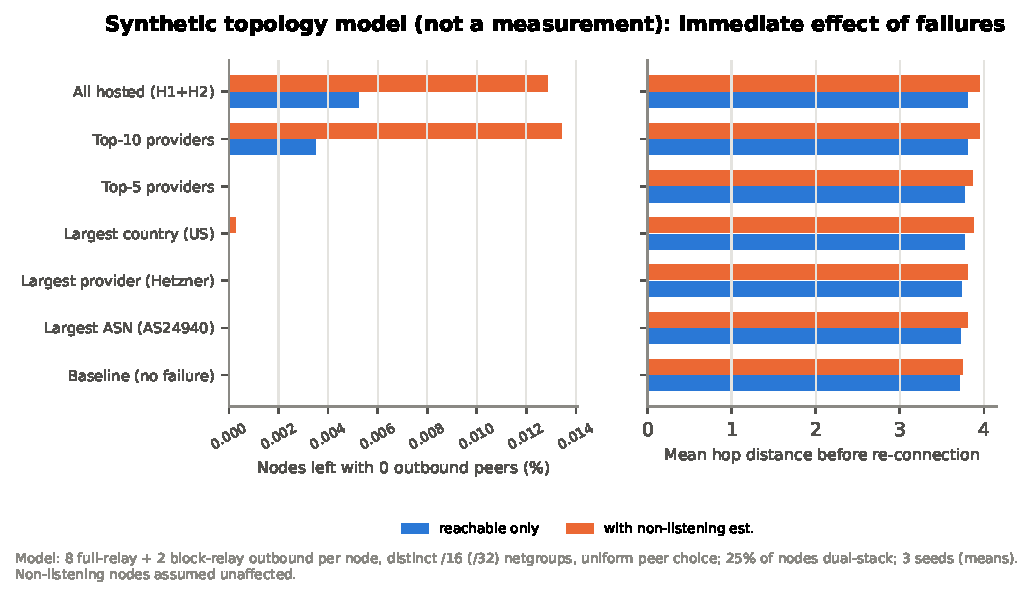
\includegraphics[width=0.95\linewidth]{failure_model.pdf}
\caption{Model results (not measurements): share of nodes left without outbound peers and mean hop distance immediately after each failure.}\label{fig:failmodel}
\end{figure}

\paragraph{Eclipse exposure.} With the default /16 netgroups, \EclNgMaj{} of modelled nodes get most of their clearnet outbound peers from a single provider, and \EclNgTopHalf{} get at least half of their full-relay peers from \EclTop. With ASN-based netgroups (\texttt{-asmap}) these shares drop to \EclAsMaj{} and \EclAsTopHalf. Nodes whose clearnet peers all belong to one provider are rare either way, \EclNgAll{} with /16 netgroups (a handful in a population of over 100{,}000) and \EclAsAll{} with asmap.

\paragraph{What the scenarios show.} The model gives no support to H2 as far as connectivity is concerned. Even the extreme and physically implausible loss of every hosted node at once leaves the rest of the network connected, because outbound connections are spread at random over thousands of netgroups and non-listening nodes connect to reachable nodes of every kind; paths become only slightly longer. Capacity is another matter. With the D4 estimate the model network is saturated before anything fails, which means that either D4 overstates the number of non-listening nodes or reachable nodes are in fact often full and the rest get by through retries, overlay networks or higher limits set by operators. Our data cannot tell these apart. Grundmann et al., however, measured that about half of reachable peers run with the default limit of 125 connections and that nearly all connection slots are in use \cite{grundmann2022degree}, which fits a network running close to saturation. What the model shows more robustly is the change. Losing a large share of reachable IPv4/IPv6 capacity, such as the top-5 providers or the largest country, adds about \UnmetRelTopfiveDelta{} percentage points of unmet demand under the defaults of released versions. Hosted reachable nodes therefore supply a good part of the capacity that the non-listening majority relies on, and in that respect H2 is partly supported. Without non-listening nodes the effect disappears. The model leaves out miner relay networks, latency and the non-uniform way in which addrman really selects peers. None of the scenarios changes the rules that the remaining nodes enforce, so losing nodes is not the same as losing control. Concentration matters most where someone acts on purpose: a provider or AS that is malicious, or forced to cooperate, could tilt the peer sets of some nodes towards itself, and in the model asmap makes this considerably harder.

% =====================================================================
\section{Dimensions of independence}\label{sec:independence}

Table~\ref{tab:independence} brings the measured values together, one row per dimension. Combining them into a single ``Infrastructure Independence Index'' would require a validated model of how each dimension affects some resilience outcome. We did not find such a model in the literature, and our data do not provide one, so any set of weights would simply reflect our own judgement. In line with the rule we fixed beforehand, we report the dimensions separately and do not compute a combined score.

\begin{table}[t]\centering\small
\caption{Dimensions of independence (functional D2 nodes unless stated). ``n/m'' means not measurable with the available sources.}\label{tab:independence}
\begin{tabularx}{\textwidth}{lXl}
\toprule
Dimension & Measure & Value\\
\midrule
Geographic & Country HHI (geoloc.) / top-1 / $N_{50}$ & \DtwoFCcHHI{} / \DtwoFCcTopone{} / \DtwoFCcNfifty\\
ASN & ASN HHI / top-1 / $N_{50}$ & \DtwoFAsnHHI{} / \DtwoFAsnTopone{} / \DtwoFAsnNfifty\\
ISP (access networks) & Share of nodes in R-class ASes & \DtwoFClassR\\
Hosting provider & Provider HHI / top-5 / $N_{50}$ & \DtwoFProvHHI{} / \DtwoFProvTopfive{} / \DtwoFProvNfifty\\
Cloud vs.\ residential & Hosted share bounds & [\DtwoFHostedLow, \DtwoFHostedHigh]\\
Software/client & Client HHI / Core share & \DtwoFClientHHI{} / \DtwoFCoreShare\\
Network layer & Share of reachable hosts on overlay networks & \DtwoOverlayShare\\
Ownership & Operators behind IPs & n/m (AS ownership $\neq$ node ownership)\\
Self-hosting & Share of reachable+est.\ non-listening nodes that are reachable & \ReachOfLukeTotal{} (D4, uncertain)\\
Outage resilience & Model, top-5 providers removed: zero-outbound share / unmet connection demand (baseline \UnmetRelBase) & \ModUTopfiveZero{} / \UnmetRelTopfive\\
\bottomrule
\end{tabularx}
\end{table}

% =====================================================================
\section{Counter-arguments}\label{sec:counter}

We set out to look for evidence against our own hypothesis, so we went through the usual objections one by one and asked whether each would change our conclusions.

\begin{enumerate}
\item \emph{Nodes at the same provider may belong to different people.} We agree, and our data cannot test it. AS2Org tells us who owns the network, not who runs the node. This weakens any reading of provider shares as ownership, but it does not affect the availability analysis, so it changes how the numbers should be read rather than the numbers themselves.
\item \emph{Concentrated hosting is not concentrated ownership.} Again we agree, and we only measure hosting (Table~\ref{tab:dimensions}). The Linode fleet (\S\ref{sec:observable}) shows that the reverse can also happen, with one operator appearing as hundreds of nodes.
\item \emph{Consensus does not require a majority of public nodes.} This is correct. Every full node validates on its own, including non-listening ones, and on its own this argument is enough to reject H3.
\item \emph{Reachable nodes are not all nodes.} D4 suggests that they are a minority. If the non-listening majority is mostly residential, our hosted shares overstate hosting in the network as a whole. We cannot check this, which is why we report two bounds (assumptions A and B).
\item \emph{Tor nodes may be missing.} We do count Tor and I2P nodes, but we cannot say where they are hosted, and they make up a large share of reachable hosts. Tor relays themselves run somewhere, and we did not measure how concentrated they are.
\item \emph{Private nodes cannot be observed.} They enter our analysis only through the D4 estimate, whose method has not been published.
\item \emph{Running a node is cheap and operators can move.} We did not measure costs. The time series does show a lot of movement, with hosted shares rising and falling by more than ten percentage points within a decade. This limits how long any dependence on a provider lasts, but it does not help during a sudden outage.
\item \emph{Cloud providers have no direct control over consensus.} This matches our analysis. A provider can switch off nodes or interfere with traffic, but it cannot change the rules that other nodes enforce.
\item \emph{Mining decentralisation and node decentralisation are different things.} We did not measure hash power. Block production can be concentrated while nodes are not, and the other way round.
\item \emph{A provider that shuts down all its nodes still does not control consensus.} The model agrees: the rest of the network stays connected, and for the largest single provider unmet connection demand rises only moderately, from \UnmetRelBase{} to \UnmetRelProv{} under the defaults of released versions.
\end{enumerate}

\noindent Objections 3, 8 and 10 lead us to reject H3. Objections 4 to 6 make the H1 estimates less certain without overturning them. None of the objections touches the finding that the infrastructure we can observe is measurably concentrated, at the provider level and even more so at the country level.

% =====================================================================
\section{Threats to validity}\label{sec:threats}

\begin{description}
\item[Crawler and vantage point.] From home, our crawler reached only \DoneIPvfour{} IPv4 nodes. When we re-probed the \ReprobeTargets{} IPv4 addresses that D2 lists as reachable but that had timed out, using 30 instead of 300 parallel connections, \ReprobeOK{} of them (\ReprobeShare) answered, which points to a saturated home NAT rather than to missing nodes. Residential nodes were lost more often than hosted ones, so D1 is biased towards hosting. We therefore repeated the crawl from an AWS EC2 instance without NAT (D1b), which reached \AwsCoverDtwoVfour{} of D2's IPv4 hosts. D1b has limitations of its own: it observes from inside a cloud provider, it started about five hours after the D2 snapshot and ran for three hours, and its IPv6 part comes from the home crawl. We keep D2 as the primary dataset because it verifies overlay endpoints and is a single consistent snapshot, and use D1b and D3 as replications. The Linode fleet also shows that crawlers differ in what they discover in the first place.
\item[Survivorship.] A snapshot only contains nodes that were online at that moment, so short-lived and intermittently reachable nodes are under-represented.
\item[Geolocation.] Geolocation and registration country agree for only \GeoAgree{} of nodes, and for \GeoAgreeHone{} of nodes in cloud ranges \cite{poese2011geoloc}.
\item[ASN attribution.] We use a single BGP view (RouteViews). Prefixes with several origin ASes affect \MoasShare{} of nodes and are assigned to the first origin. KIT's ASNs come from its own whois lookups.
\item[Classification.] Classes assigned per AS do not necessarily describe individual hosts \cite{ziv2021asdb}, which is why we report bounds. The name-based rule produces some false positives and affects \RegexShare{} of nodes.
\item[Duplicates, NAT and dynamic addresses.] Counting by IP merges several nodes behind one NAT and splits a node whose address changes. At the /24 level there are \DtwoFSubnetGroups{} distinct subnets and the largest holds \DtwoFSubnetTopone{} of nodes, so clustering within subnets is small.
\item[Tor, I2P and IPv6.] Overlay nodes cannot be attributed, and IPv6 attribution depends on a smaller BGP table.
\item[Private nodes and stale data.] Non-listening nodes enter only through D4, and the attribution sources are up to 33 days older than the node data.
\item[Change over time.] The KIT series shows that these distributions change over the years, and our two measurement days show that individual nodes turn over within days even when the distribution stays put. Two days are still a short window, and our results describe October 2026.
\item[Time series.] Organisation names and classes for 2015--2025 are taken from 2026 sources, so an AS that changed owner or business is classified by its current state.
\item[Model.] Random peer choice, a fixed share of dual-stack nodes and the absence of miner relay networks are simplifications, and the model's outputs are not measurements.
\end{description}

% =====================================================================
\section{Discussion}\label{sec:discussion}

\paragraph{What we observed.} Among nodes that can be attributed, the provider HHI is about \DtwoFProvHHI{}, the largest provider hosts about \DtwoFProvTopone{}, half the nodes are covered by about \DtwoFProvNfifty{} providers, the country HHI is about \DtwoFCcHHI{}, and between \DtwoFHostedLow{} and \DtwoFHostedHigh{} of nodes are hosted. Bitnodes, KIT and our own AWS crawl all produce very similar figures, and repeating two of them two days later changed the provider HHI by at most \TdMaxProvHHIChange{} points.

\paragraph{How we interpret it.} Concentration exists and can be measured (H1), but at the provider and AS level it is moderate and has decreased since 2020. Losing several large providers at once would remove a substantial part of the reachable IP nodes without, according to the model, splitting the network (H2 not supported for connectivity). It could, however, push the remaining reachable nodes beyond their inbound capacity, to an extent that depends on how many non-listening nodes there really are (H2 partly supported for capacity). Hosting concentration does not give anyone control over consensus (H3 rejected). The more relevant risk is deliberate interference by an AS or provider that biases peer selection or intercepts traffic \cite{apostolaki2017hijacking,tran2020erebus}. In that context, the fact that ASN-based bucketing exists but is not enabled by default deserves attention.

\paragraph{Limitations.} The nodes we can attribute are a minority of all nodes, we cannot see who operates them, and the topology is modelled rather than measured.

\paragraph{Open questions.} Two hypotheses remain untested: that most non-listening nodes are residential, and that the infrastructure behind Tor relays is concentrated in the same way as node hosting. Testing either would require data we do not have.

% =====================================================================
\section{Conclusion}\label{sec:conclusion}

The Bitcoin nodes we can observe are measurably concentrated on several infrastructure dimensions, most strongly by country and less so by AS and hosting provider, and the concentration is lower in 2026 than it was in 2020--2022. The evidence does not support the stronger claims that this concentration threatens the network's connectivity or hands control over consensus to infrastructure owners: in our model the network stays connected even without any hosted nodes, and nodes on different chains share the same providers. The weaker point is capacity. Reachable nodes, a small minority of all nodes if the D4 estimate holds, carry the connections of everyone else, and losing many of them at once would shift that load onto the rest.

Several of our findings concern measurement as much as the network itself. Most reachable nodes cannot be attributed to any infrastructure, a single fleet or a single vantage point can change the headline numbers, and node counts include nodes that follow different consensus rules. We think infrastructure concentration is best understood as part of Bitcoin's attack surface, to be addressed through peer diversity mechanisms such as ASN-based bucketing, and not as a measure of who controls Bitcoin.

\paragraph{Use of AI tools.} The measurement and analysis code (crawler, data download and attribution pipeline, metric computation, topology model, figure and table generation) was developed with the assistance of the large language model Claude Opus 5.5 (Anthropic), used through Claude Code. The model also assisted with drafting the manuscript text and with automated checks of bibliographic metadata against Crossref. All outputs were reviewed by the author, who takes full responsibility for the methodology, the data, the results and their interpretation. The model is not an author of this work.

\paragraph{Data availability and ethics.} Many node operators run nodes from home, which makes node addresses (IPv4, IPv6, onion and I2P) personal data, so we do not publish them. In the public release every address, subnet and netgroup is replaced by a pseudonym computed with a keyed HMAC-SHA256, and the raw crawl and Bitnodes files are left out. We checked that running analysis steps 05 to 08 on the pseudonymised data reproduces every number in this paper. Our crawler only performed the standard handshake and address exchange and identified itself with an honest user agent.

\paragraph{Reproducibility.} The code, the hashes of all raw files and the derived tables are in the accompanying repository. The numbered scripts in \texttt{analysis/} reproduce every number in the paper, and the numbers in the text are generated macros (\texttt{paper/numbers.tex}).

\bibliographystyle{plainnat}
\bibliography{references}

\end{document}
